\section{Attributing an Issue to a Column Group}
\label{app:attribution}

% VALUE: the one disclosure in the paper that a reviewer should be able to audit in full: the attribution rule was
% settled after the capture, the earlier rule labels the same capture differently, and the evidence that the later
% rule is the physically right one comes from waits and argument slots rather than from the rule itself
Because FastFlowLM's attention reads through shim tiles of the GEMM columns, the analysis attributes each issue to the column group whose compute tiles its data reaches through the decoded routes, not to the column the instruction addresses (Appendix~\ref{app:capture}).
This appendix states how that rule was chosen,
because it was settled after the capture it is applied to and the earlier rule gives a different label.

\textbf{Why the addressed column is not the group.} In the production engine's fused prefill, each attention command
also pushes one shim queue on a column belonging to the other group: one image pushes on column~6 and another on
column~3. Attributing those pushes by the column they address places them in the GEMM group, inside commands that are
otherwise attention, which yields 10{,}822 group transitions of which 10{,}752 are internal to a command.

\textbf{Why those pushes belong to attention.} The evidence is independent of the attribution rule. The two images'
synchronizations are on the attention column only: 128 waits all on column~7 for the first, 256 all on column~0 for
the second, and no GEMM image touches column~0 or~7 at all. The borrowed channel reads a different argument slot than
the attention column's own while carrying that slot's exact per-block pattern, which is a second input streamed in
lockstep rather than GEMM work. The route itself is in the configuration, not in the control code.

\textbf{The two labels.} Under the rule registered first, by addressed tile column, the capture is mixed, with 99.4\%
of its transitions internal to a command. Under the rule the paper uses, where each issue takes the group whose compute
tiles its data reaches by the configuration's routes, the capture has 70 transitions, 35 into attention and 35 out of it,
and every one sits at a boundary between two commands, which is the serial label. We record plainly that the second
rule was proposed after the capture and moves the outcome toward our claim: under the rule registered first, the
compute-weighted share of the transitions of the overlapping kind is 0.776 (its bytes-only share 0.912), which is the
majority-mixed label, so the serial prediction we registered was a miss under the registered instrument and a hit
only under the rule chosen afterwards.

\textbf{What a population check adds, and what it does not.} Over all 218 recorded streams, the columns that carry any
instruction fall into four sets: 200 streams address only the GEMM columns, 8 address columns $\{0,3\}$ and 8 address
$\{6,7\}$, 1 addresses all eight, and 1 carries no instruction. In the capture itself, 276 of 311 commands address only
the GEMM columns, 28 are one image on $\{6,7\}$ and 7 the other on $\{0,3\}$, and the stream that addresses all eight
is not dispatched. In every two-column stream the bulk of the instructions sit on the attention column, by 1{,}420
against 384 in the largest case. This counts addressed columns and not the programs those instructions serve, so it
corroborates the attribution rather than establishing it; and because a rule that labels each command by the
columns it addresses also gives 70, the fact that the column set changes exactly 70 times re-derives that count
rather than measuring it a second time.

\section{Other Round-Trip Populations}
\label{app:roundtrip}

% VALUE: the lead contribution's number will be audited, so the populations beside it are stated rather than left for
% a reviewer to find
The 625 streams quoted in the introduction are the streams each toolchain emits for a design. Three further
populations round-trip byte-identically and are not counted there, to keep that number tied to one kind of object.
The open compiler also dispatches streams that differ from its on-disk files, either stripped to a column group or
interpolated from a template: 539 of those re-emit byte for byte, and none of them is among the 375, so that toolchain
has 914 distinct streams verified across two gates. Our own composer's output re-emits on 2{,}684 streams, which we
exclude from a toolchain count because it is our output rather than a stack's. The production engine's streams at
other prompt lengths, 37 and 53 in two further gates, overlap the 218 already counted. Each gate carries two negative
controls, a modified stream and a truncated one, which fail as designed.

\section{The Production-Engine Comparison}
\label{app:flm}

% VALUE: the inequalities behind the reference point, and an honest statement that we can price only part of the gap
The comparison with the production engine in Section~5.2 is a reference point, not a like-for-like speedup. The two
stacks differ in their kernels, their dequantization path, their tokenization, and the chunk size their prefill uses,
and we hold the weights and the prompt fixed but not those.

\textbf{What we can price.} In a capture of the engine's dense path at two prompt lengths, the command counts are
fixed: 146 commands, 64 configuration switches, 12 module and kernel constructions and 226 runs per request at both
lengths. A separate dequantization pass is fixed in count and in time, 16 run lists of four commands taking
78--84\ms{} at both lengths, and one further pass takes 18--20\ms. That is about 100\ms{} of fixed device time, which
is 40\% of the 248\ms{} difference from the shipped program at 2{,}048 tokens and 49\% of 208\ms{} at 4{,}096. Every command in the capture is
serial, and the unit repeated per layer is a dequantization, three matrix multiplications, an attention command and
four more matrix multiplications.

\textbf{Where the difference goes.} Recording both stacks the same way, by the time each command is outstanding on
the device and the time the host spends with nothing outstanding, accounts for the whole of the difference at a
4{,}096-token prompt, where the difference from the shipped program with attention alternated was 194\ms{} on the days of the two recordings. Host time accounts for more than all of those 194\ms{}: the production engine spends 318\ms{} with no command
on the device against our 96\ms. Its fixed passes account for a further 102\ms. Its matrix work runs 65\ms{} longer
than ours. Against those, its attention runs 196\ms{} \emph{faster} than ours, which is the one place the hand-tuned
engine is ahead of the design we rewrite, and which is why the difference is not larger.

Two limits on that accounting. The comparison is by command kind rather than by identical work: our matrix figure
includes the LM head and the dequantization folded into each multiplication, which the engine pays
elsewhere. And the recording locates the host time without seeing into it, since the interposer observes the gaps
between calls rather than what runs inside them, so the dominant term is host-side time we can place but not
decompose. At a 2{,}048-token prompt we have no equivalent record of the open stack and attribute nothing.
% SOURCE: vault lab-flm-streams (15), no device. FastFlowLM from the capture's serial issue-to-done per kind; the open
% stack from the ML Timeline hold-2 records, 1B shipped with attention alternated at 4,096 tokens, TTFT 1,607.6 ms,
% per-command first issue to last return unioned per column group, median of 5 reps: GEMM group 895.0 ms, attention
% group 617.1 ms, overlap 0.0, host time with nothing outstanding 95.6 ms. FastFlowLM: GEMM 959.9, attention 420.8,
% separate dequantization and layer passes 102.5, host idle 318.5. Differences +64.9, -196.4, +102.5, +222.9, summing
% to +194.0 against a measured window difference of 194.1 on these two days. The two sides come from different holds
% on 2026-10-21.
\section{Registered Predictions: Flagged Arms}
\label{app:flags}

% VALUE: the arms whose spread or bracket exceeded its threshold, listed so that a reader can see that none is a
% composer arm and that all were scored as they stand
Four baseline arms varied by more than 5\% across their repetitions: the shipped program at 12{,}288 + 2{,}048 tokens on
one split of Llama-3.2-1B (+6.3\%), the shipped program at 2{,}048 + 4{,}096 on another split of the same model
(+6.7\%), and at 2{,}048 + 4{,}096 on Qwen3-4B both the shipped program (+8.4\%) and the shipped program with its
attention columns alternated (+5.8\%). One bandwidth bracket, on a Gemma3-4B split that the composer does not choose,
ran 7.3\% above the day that split's probes were taken; it touches only comparisons at that split, and the split the
composer chooses for Gemma3-4B is the other one throughout. No composer arm was flagged. Every flagged arm is scored
as it stands, and none was re-run after its outcome was seen.

\section{The Synthetic Designs}
\label{app:synthetic}

% VALUE: the three disclosures that belong with the synthetic measurements, including the one hold whose bandwidth
% bracket is missing and an observation the registration did not anticipate
Three disclosures belong with Section~5.4's synthetic designs.

First, in the all-or-nothing design at the smallest level of core work, the repetitions of the depth-one baseline span
193\% of their median, because that variant was the first opened in the hold; its median is the statistic the
registration names, and the other spreads in that design are between 0.4\% and 4.9\% except three, of 34\% at the same level and 15\% and 14\% at the middle one.

Second, the bandwidth cap probe did not run for that hold, because a relative output path was passed to a probe that
changes directory first, so no cap reading brackets those measurements. It is not one of the output checks, all of
which passed. The other two holds read 13.4--13.5~GB/s at one column and 54.7--55.1~GB/s at eight columns at both ends.

Third, an effect we did not anticipate and can now account for: in the order-by-loop
design at buffer depth four, both orders run at 11.65\ms, 3.2 times the depth-two time of the faster order, where a first
reading of the period had expected the two depths to agree. We did not alter the design after measuring it. No cycle of the depth-two graph accounts for it, since adding buffer slots can only add tokens to a cycle
and cannot raise any cycle's mean, so the firing times themselves differ at depth four. Comparing the final
configuration state of the four built designs localises that: every shim-tile and memory-tile register is identical
between the depths, with no change to a transfer, a route or a lock outside the cores' own tiles. Reading the lowered
code names it. The buffer selection lowers to a two-way choice between constants at depth two and to a load from a
three-entry table of addresses at depth four, and the inner loop over 1{,}024 elements is unrolled at both depths but
software-pipelined only at depth two: 12 instruction bundles per four elements against 38, with each load at depth four
waiting out its latency. Those counts predict 6.29 and 19.92 million cycles, which match the measured 3.610\ms{} and
11.653\ms{} at 1.74 and 1.71\,GHz against an 1.8\,GHz clock, so the bundle counts account for the slowdown to within
2\%. Why pipelining stops is not established; a pointer loaded from a table cannot obviously be proven not to alias the
input, which would block hoisting loads above stores, but we did not check that, and we have not excluded the memory
banks the depth-four buffers share. What the certificate compares is unaffected, since both orders at depth four run
the same loop; what changes with depth is the time of that loop, and the mechanism for it is named above.

\section{Reference Checks and the Gemma3-4B Gate Result}
\label{app:gemma-gate}

% VALUE: the three instruments differ in kind, which matters more than how many tokens each covers; then the 1B
% result that clears the headline model's prefill path, then the Gemma result with its scope
Three kinds of instrument are available to us, and they are not interchangeable. The expected continuations shipped
with the Qwen3-4B and Gemma3-4B modules are constants their authors recorded from their own device runs, one of them
re-recorded after the authors fixed a bug that had zeroed a feed-forward contribution; agreement with such a constant
is a regression check against the authors' output over ten tokens, not a statement of numerical fidelity. The
remaining instrument is a floating-point forward on the same quantized weights, which two of the stacks provide and
which the designs are themselves gated against; comparing to it detects drift of the device's arithmetic from that
forward, and it is the instrument used for the two checks below. It is not an independent implementation of the
model, and we do not claim it as one.

\textbf{Llama-3.2-1B.} Against that forward, the shipped prefill's keys differ by 0.4--3.0\% and its values by
1.1--7.5\% across the sixteen layers, on a six-token prompt and on a 256-token one, and the two split builds give the
same errors to every digit we report. The error grows over the first eight layers and then holds, with no step of the
kind the next paragraph describes. The first token matches the forward's on both prompts and both builds. Seeding the
turn's decoder from the forward's own keys and values, from one split's, and from the other's produces the same
seventeen tokens in all three cases, so these differences do not change what decode emits. All three agree with the
forward's own continuation for ten tokens and then differ, at a step where the forward's margin between its top two
tokens is 0.16, its second-narrowest in that sequence; because the difference appears even when the decoder is seeded
from the forward's own keys and values, it lies between the device's decode and that forward rather than in the
prefill we rewrite.

\textbf{Gemma3-4B.}

% VALUE: the per-layer detail behind the body's statement that one configuration fails a reference check, with the
% scope stated so that it cannot be read as either our build being broken or the stack being inaccurate
Section~5.1 reports that we measure no turn on Gemma3-4B because the configuration failed a reference check before any
run was timed. The check crossed two sources of keys and values, the module's own reference forward and the path the
turn harness uses, with two decode paths, on a six-token prompt with nine greedy dispatches.

Both reference-sourced arms reproduce the reference continuation exactly, and for either source the two decode paths
give logits that agree bit for bit, so both decode paths and the seeding step are clean. Both arms sourced from the
split path diverge at the fifth decoded token, with the same continuation the turn run produced. The keys
differ from the reference by 0.6--1.8\% in layers 0--9 and 5.0--9.1\% in layers 10--33, and the values by 0.8--4.9\% in
layers 0--31 and by 6.8\% and 13.0\% in the last two. The divergence lands on a near tie: with the reference's keys and
values the correct token leads by 0.875, and with the split path's the other leads by 0.25.

Two further measurements bound what this result is. The two floating-point forwards available for this model, the
one used above and the stack's other, agree with each other to 0.3--1.1\% on keys and 0.2--1.7\% on values, and give
the same first token with the same five leading candidates in the same order, so the difference reported here is five
to nine times the disagreement between the instruments and is not an artifact of which one served as the oracle. It
is also not of a different order from this stack's usual quantization error: on Llama-3.2-1B the shipped prefill
differs from its own forward by up to 3.0\% on keys and 7.5\% on values without changing a single decoded token. What
distinguishes this case is that the larger difference fell on a near tie.

The keys and values that fail came from the shipped prefill program, with no rewrite of ours applied, and were
stacked by the compiler's own routine. Two comparisons settle where the difference comes from. The build our harness
uses is the module's own program: rebuilt by the module's own builder, in the same checkout and without opening the
device, 22 of its 38 files are byte-identical and the remaining 16 are identical in size with their differences
confined to header identifiers and a timestamp, which do not reproduce between builds. The same holds for the two
models that carry our decode and turn results: rebuilding the baseline prefill behind every reported run of
Llama-3.2-1B, at both window sizes, and of Qwen3-4B gives 18 of 30 files byte-identical and the 12 remaining of equal
length with byte-identical images, differing only in those same identifiers. So the program we compare against is the
module's own on every model we report. This covers the baseline split alone, since the other two splits are
constructions of ours and have no counterpart to rebuild. And the keys and values do not
depend on our host path: the in-tree build loaded by the module's own path, the split build loaded by that path, and
the split build loaded through our turn harness with its specification patch, its weight arenas and its template
produce keys and values bit-identical to one another, with a maximum absolute difference of zero, each reproducing
the error above to the digit. The first attempt at this comparison did not run: its own floating-point reference step raised the machine's
load average above the threshold the protocol requires before the device is opened, and it exited at that check
before any device was opened; the comparison was repeated after a wait for the load to settle.
The difference is therefore the shipped program's own. We claim no cause for its step at
the tenth layer, and we report this model's prefill results as measured, taken on that program and producing its own
keys and values. The comparative claims elsewhere in the paper are untouched, because they compare a rewrite with the
shipped program on one build.

\section{Choosing the Split Before Reordering}
\label{app:split-first}

% DECISION: relocated from the introduction's list of reasons the loss survived (decisions log D19g, 2026-10-22): under the stronger baseline the existing program's faster split agrees with the composed one in 8 of 8 W1 cells and 11 of 12 Table 4 cells, so it is a narrow finding rather than a reason; kept whole, not deleted.
Tuning the array's partition before reordering issue rarely leads somewhere other than the partition the reordered program wants. Without the hand alternation, the faster split for the shipped program is not the one the reordered program wants at three of the configurations we measure; interleaving the shipped program's own attention columns by hand removes those three, but on Llama-3.1-8B, for a 4{,}096-token append to a 4{,}096-token context, the interleaved program still runs faster with four attention columns where the reordered one wants two.
% SOURCE: the un-alternated shipped program prefers S4 while every reordered version prefers S2 at 1B scratch 2,048 / 4,096 and Qwen3-4B scratch 4,096 (5-rep w1 files, vault paper-cosched-claims-v2, lab-split-sweep (18)); Llama-3.1-8B 4k + 4k: shipped S4 10,909 ms, shipped + Ar S2 11,440.1 ms, shipped + Ar S4 = shipped S4 (the alternation is a no-op on S4), composer S2 7,395.4 ms (lab-split-sweep (14), (20)). Corrected in the 2026-10-22 foundation audit (B14): the earlier clause said the two agree once alternated.


\section{Registered Predictions and Their Scoring}
\label{subsec:tests}

% VALUE: every prediction is tested as registered before its run: the bound against every measured removal, the event model's times, the joint prediction, and the composite test with its expected outcome stated beforehand; counts reported in full
Every quantity this section computes is predicted before the run that measures it, in a registration committed to the repository, and scored afterwards by a program fixed at the same time.
Four predictions test the event model: which split is faster at each configuration, the sign of every pairwise comparison between schedules, the absolute error of each predicted time against a tolerance stated in advance and against a linear interpolation between measured configurations, and the end-to-end gain.
Two test the bound: that no measured gain exceeds the bound computed for it, and that the composed schedule stays within a stated distance of the bound.
One tests the renaming of the decode loop, as a band on the per-token gain at two context lengths rather than a point.
One tests the set property directly, on designs written to hold two name dependences at a known position: that a removal off the binding cycle is worth nothing at every level of core work, with that outcome, and not a gain, stated as the prediction.
Section~\ref{sec:eval} reports each outcome with its counts, including the three that failed and the direction of each failure.
% DECISION: the outcomes and the verbs they allow follow outline v9 section 3's rows; a test not completed is reported as its least favourable outcome.
% SOURCE: the inventory is the set actually scored: the event model's four (Section 5.2, E1-E4, with E4 failed), the bound's two (Section 5.7, the 33-run check held and the 1.30x range failed on 5 of 12), the decode band (Section 5.5, both cells in band on Llama-3.1-8B), and the synthetic certificates (Section 5.3, held at two of three work levels). Nothing else in the paper is registered, and this list is re-checked against the scores at the results freeze.

\section{Discussion}
\label{app:discussion}

% MERGED from the former discussion section
% VALUE: transferable insights only, each a possibility under its condition and tied to a measured result: an in-order issuer rations concurrency so its order is the schedule and packing yields little of it; the faster partition may change with the regime, so evaluations of prompts from scratch only may choose the wrong one; probes may rank configurations reliably before they run; once ordered, the bound may move from the issuer to the groups; a false dependence inside an operator is out of reach of reordering but not of renaming; on agent turns, gains measured from scratch may misstate end-to-end gains
Although we evaluate one NPU, our findings rest on properties that other spatial accelerators may share.
Where an in-order issuer mediates the concurrency of an array, its instruction order may act as the schedule, so packing work into fewer dispatches may yield little concurrency, and a second queue or a completion signal per group of columns could remove the rationing in hardware (Sections~\ref{subsec:semantics} and~\ref{subsec:ablation}).
Where operators are partitioned spatially, the faster partition may change between computing a prompt from scratch and appending to a cached context, so an evaluation of prompts computed from scratch alone could choose the partition that is slower for agents (Section~\ref{subsec:ablation}).
Where issue returns at once and waits block, probes of each operator alone may rank configurations reliably even where they misprice them, so a configuration can be chosen before it runs (Section~\ref{subsec:accuracy}).
Once the issue order is right, the binding term may move from the issuer to the groups' own busy time, so further gains could come from kernels and from the balance of work between groups rather than from scheduling (Section~\ref{subsec:bound-eval}).
Where an operator reuses one buffer across the iterations of a loop, reordering issue across operators cannot reach the resulting wait, whereas renaming the buffer inside the operator could (Section~\ref{subsec:decode-eval}).
Finally, where agents append to long contexts, prefill becomes bound by attention and decode by the KV cache, so gains measured on prompts computed from scratch may misstate what an agent's turn gains (Section~\ref{subsec:turns}).
% DECISION: each sentence is re-checked against its section's result at the results freeze; a sentence whose result does not hold is dropped (vault paper-cosched-plan, section 6).

% The former limits paragraph is distributed to the points it qualifies: the passes' scope to the passes, the
% host state to the turn result, the reference-point caveat, the gates, the composition cost and the two failed
% predictions to the evaluation, and the analysis's refusals to the analysis. Only the one-device limit, which
% qualifies the transfer argument above, stays here.
We measure one generation of one vendor's array, so the transfer above rests on the properties we name rather than on measurements elsewhere.

% VALUE: the ownership consequence of the placement in Related Work: the program, and so the compiler, owns concurrency across column groups as in Rammer; a device reading busy while one group works shows why; other in-order arrays may share the property where their streams can be read
On XDNA~2, one in-order CP per hardware context leaves to the program the job that hardware queues do on a GPU since Kepler (Section~\ref{sec:related}), so the compiler owns concurrency across column groups, much as Rammer's compile-time schedules do on GPUs and IPUs~\citep{ma2020rammer}.
A device that reads busy for 92--97\% of TTFT while only one column group works at a time shows why this ownership matters, since utilization measured per device hides the idle columns (Section~\ref{subsec:losses}).
Other arrays whose engines run their programs in order, such as other AIE generations, may share this property, so the same analysis could apply where their streams can be read.
% SOURCE: device busy = summed isolated operator times less the dispatch floor, 92/95/97% of TTFT at 512/2k/4k (amd-npu e3acc8a, Figure busy), not a hardware counter.
% DECISION: "the compiler owns concurrency on static hardware" is cited (Rammer, TSP) and kept as discussion, never a contribution (outline v9 section 2, "Not contributions").

\section{Further Related Work}
\label{app:related}

% VALUE: orientation: the related work of the body in full, with the works and detail its run-ins leave out
% DECISION: verbatim from the former Related Work section (aie-cosched 548aa83, 9-related.tex); the author prunes what the body already carries.
This section gives the related work of Section~\ref{sec:related} in full, including the works and detail that its run-ins leave out.

\textbf{Statically Ordered Accelerators.}
% VALUE: other machines fix order or timing in the compiler (TSP: timing; ReGate: compiler-managed idleness for energy; Rammer: a compile-time schedule on GPUs and IPUs); on XDNA 2 only the order is fixed by the program, across asynchronous engines
Groq's TSP removes reactive hardware such as arbiters and caches so that its compiler determines when every instruction executes~\citep{abts2020tsp}.
ReGate power-gates the components of an NPU, with a compiler that manages the idle periods of vector units and SRAM through ISA extensions and hardware idle detection for the inter-chip interconnect and memory controllers~\citep{xue2025regate}.
Rammer generates a static spatio-temporal schedule of a DNN's operators at compile time on GPUs and IPUs, instead of relying on a second, run-time scheduler~\citep{ma2020rammer}.
On XDNA~2, the program fixes the order of each engine's work and the waits between engines, whereas the durations of the DMA, core, and CP engines are not fixed, so the order can be read from the shipped program while time remains a measured input.

\textbf{NPU Compilers and Deployments.}
% VALUE: compilers, mapping frameworks, and hand-tuned runtimes decide what a design computes and where, and NPU schedulers reorder command graphs or split work across devices from their own models; our setting analyses designs already compiled, open and closed
MLIR-AIR and IRON compile operators and fused multi-operator designs onto the AIE array~\citep{wang2026mlirair,hunhoff2025iron}, and Stream explores layer-fused mappings on multi-core dataflow accelerators with memory- and communication-aware cost models, emitting one design per fused group on its AIE backend~\citep{symons2025stream}.
A FlashAttention case study on XDNA NPUs maps the fused kernel by hand and uses a roofline per memory level to decide when to stop fusing~\citep{wang2026flashattention}.
FastFlowLM runs many model families on XDNA~2 NPUs with hand-tuned designs~\citep{fastflowlm-repo}, and its authors' Gemma3 mapping double-buffers the keys and values of decode attention~\citep{du2026gemma3}.
MLIR-AIR also builds end-to-end decoder models from fused operator designs, and in both stacks the composition of operators into commands and the split of the array are fixed by hand for each model.
TileFuse fuses mixed-precision dequantization into the GEMM kernels of XDNA~2~\citep{pang2026tilefuse}, and an agent skill system deploys decoder models end to end through MLIR-AIR~\citep{li2026agentnpu}.
A line of work automates the mapping itself: ARIES compiles for AI Engine devices through MLIR with an abstraction for their levels of parallelism~\citep{zhuang2025aries}, Allo separates compute, memory, communication and data-type customizations from the algorithm and composes them across a design's hierarchy~\citep{chen2024allo}, Dato expresses a program as a graph of tasks joined by explicit stream types and sharded by layout types, mapping them onto the spatial fabric and then onto the hardware's limits, and reports utilization and attention speedups on this NPU against IRON~\citep{fang2025dato}, and AIE4ML compiles quantized networks end to end into firmware for this generation of the array~\citep{danopoulos2025aie4ml}.
On mobile NPUs, llm.npu offloads prefill through chunked static graphs and runs outlier channels on the CPU~\citep{xu2025llmnpu}.
LATTICE reorders NPU command graphs taken from traces jointly with memory planning and reports a modeled makespan~\citep{liu2026lattice}, whereas HeteroMosaic and Agent.xpu schedule LLM work across the CPU, GPU, and NPU of one SoC~\citep{jun2026heteromosaic,wei2025agentxpu}.
These works decide what a design computes and where it runs, or how a given command graph is ordered, and each generates a design from a program it is given. Dato is the closest to our subject, since its tasks carry explicit streams and are placed on the fabric, but like the others it compiles a design rather than reading one back.
LATTICE is the closest on the question we ask, because the last of its three stages sets out to recover pipeline parallelism, and it differs from us in its input and in its evidence: it orders a command graph taken from traces and reports a modeled makespan, whereas we recover the ordering from the instruction streams a stack emits, re-emit 625 of them byte for byte to establish that the reading is faithful, and measure each removal on the device with outputs bit-identical to the design we rewrite. Our setting takes compiled designs as given, including one we cannot recompile, and concerns the dependences inside and between them on one array.
% SOURCE: LATTICE (arXiv 2607.17422v3, abstract read 2026-10-22): three stages, memory-pressure-aware topological
% scheduling, deterministic linear repackaging for placement and spills, and critical path enhancement for
% recovering pipeline parallelism; six command traces from a DaVinci NPU; reports peak memory, extra DDR traffic,
% spill count and modeled makespan. A search surfaced this eprint under the title "DAN-Scheduler"; the live arXiv
% record is LATTICE with the eight authors our entry already carries, so there is one paper and no second citation.
% SOURCE: FlashAttention case study's stop-fusing rule and ridge points (vault src-xdna-flashattention-study); FlowKV in 2602.06063 section 4.1 and 3.2.3, full text checked by review r14 (vault src-gemma3-edge, outline v9 section 2); Stream describes no switching cost and no concurrency across fused groups (vault src-stream-dse, arXiv v2 read 2026-10-14).

\textbf{Performance Prediction and Attribution.}
% VALUE: what-if tools take the order from traces and simulate transformed graphs, causal profiling measures a line's worth by experiment, GPA attributes stalls within GPU kernels from PC samples, cost models and WCET analysis predict or bound execution time, and command streams have been captured from a closed GPU driver; none takes the order between asynchronous engines from the program or bounds the worth of removing one ordering
Daydream and dPRO build dependency graphs from run-time traces and simulate transformed graphs to predict what an optimization gains~\citep{zhu2020daydream,hu2022dpro}, and Habitat predicts a model's training time on one GPU from a run on another~\citep{yu2021habitat}.
Coz measures what speeding up a line of code would gain by slowing down all code that runs concurrently with it~\citep{curtsinger2015coz}.
GPA attributes sampled GPU instruction stalls to their causes by data-flow analysis within a kernel and estimates the speedup of each suggested fix~\citep{zhou2021gpa}.
Learned and analytical models predict the time of a tensor program or of a mapping on an accelerator~\citep{kaufman2021learned,parashar2019timeloop,kwon2019maestro}, and WCET analysis bounds the execution time of a binary statically~\citep{wilhelm2008wcet}.
Command streams have also been recovered from a closed GPU driver to attribute runtime behavior~\citep{yan2026revealing}.
These tools take the order of operations from a trace, or predict or bound execution time, whereas the order between the NPU's engines is fixed by its program, and the quantity we bound is the worth of removing one ordering.

\textbf{Pricing a Change Before Building It.}
% VALUE: the worth of removing an ordering is a classical question: project crashing cuts the critical network, retiming and modulo scheduling reason about the recurrence bound, causal profiling measures a line's worth by experiment, and trace-based simulators replay a design to price a change; our setting takes the graph from a compiled binary of a stack we did not compile, and the shared DRAM cap means a cut of the critical path is necessary but not sufficient
Shortening a project by cutting its critical network is a classical problem whose optimal reduction is a minimum cut of that network~\citep{kelley1961critical,fulkerson1961network}, and the throughput of a cyclic dataflow graph is set by its maximum cycle mean, which state-space and cycle-mean analysis compute~\citep{ghamarian2006throughput,stuijk2008throughput}.
That bound on a recursive graph is computable in polynomial time~\citep{gerez1992iteration}, and exact formulations select the combination of retiming, c-slow retiming and recycling that optimizes the resulting performance~\citep{bufistov2007general,bufistov2009retiming}.
Causal profiling instead measures what speeding one component is worth by experiment, and its motivating case is that speeding one of several parallel paths gains nothing~\citep{curtsinger2015coz}.
Interaction-cost analysis defines a bottleneck as a set of events, costs it by the time saved when the whole set is idealized, and identifies the case where each member alone saves nothing while the set saves~\citep{fields2003interaction}.
We take that set view of a bottleneck as given, and our subject is which sets a compiler may legally remove from a shipped binary, and what the shared DRAM cap then leaves of the saving.
LightningSim replays a trace of a high-level-synthesis design and recomputes its longest paths incrementally, so that the effect of a change is priced before the design is rebuilt~\citep{sarkar2023lightningsim,sarkar2024lightningsim2}.
We take the graph from a compiled binary, including a stack we did not compile and may not modify, and on this machine the column groups share a DRAM read cap, so cutting every critical path is necessary for a removal to pay but not sufficient.
% SOURCE: the acyclic condition is project crashing's minimum cut of the critical subnetwork (Kelley 1961; Fulkerson 1961); the cyclic condition is the iteration bound and maximum cycle mean (Ghamarian 2006; Stuijk 2008). Gerez, Heemstra de Groot and Herrmann 1992 give the polynomial-time iteration-period bound (read 2026-10-21: the paper computes the bound; it does NOT compute the next-critical loops, so that property is not attributed to it); Bufistov et al. ICCAD'07 is the exact ILP model over retiming, c-slow retiming and recycling, and DAC'09 the MILP for elastic systems with early evaluation.

\textbf{Compile-Time Synchronization and Binary-Level Analysis.}
% VALUE: other work places synchronization while a kernel is lowered, or needs a trace and a simulator to study what ran; we read the synchronization already present in a shipped binary, including one we did not compile, and bound in time what removing a given wait is worth; minimizing the count of synchronizations is a different objective from removing a wait that costs time
The auto-sync feature of AscendNPU-IR inserts a kernel's synchronization as it lowers, deciding set and wait pairs from a memory-dependence analysis over its own intermediate representation and dropping redundant pairs so that the fewest hardware events are used~\citep{ascend-autosync}.
xPU-Shark records traces from production accelerator deployments and replays them in a microarchitecture simulator, which lets it analyze a deployed model at the level of machine code~\citep{zarkadas2025xpushark}.
These approaches place synchronization while a design is compiled, or study what ran from a trace and a simulator, whereas our analysis reads the synchronization already present in a shipped binary, including one that we did not compile, and bounds in time what removing a given wait is worth.
Using the fewest synchronizations is also a different objective from removing a false dependence: a wait that a stack needs is not redundant, even where its position holds one column group behind another.
A vendor compiler may also report a cost for what it has just produced: Arm's compiler for its Ethos-U NPUs prints an estimated cycle count per layer for a compiled network, and Arm's documentation states that those numbers exist for the compiler's own optimization decisions, should not be taken as accurate representations of real performance, and should not be compared across compilations, directing anyone who needs performance to an FPGA or a virtual platform~\citep{vela-performance}.
% SOURCE: Vela PERFORMANCE.md ("Vela Performance Estimations"), read 2026-10-21: "The cycle and bandwidth numbers should not be taken as accurate representations of real performance numbers"; "The numbers reported allow the compiler to make its optimisation decisions only"; "For accurate performance numbers the network should be run and profiled on an FPGA."
We report a narrower quantity for a different purpose: the time that removing one named wait is worth, which decides whether a rewrite is attempted at all, and which we then check against measurement on the device.

\textbf{Dependences and Dataflow Analysis.}
% VALUE: the dependence classes, renaming, software pipelining, scheduling with a common server, and SDF throughput analysis are established and cited; they take the program or graph as given, whereas here the graph spans asynchronous engines and is recovered from compiled instruction streams
Compilers distinguish flow dependences from anti and output dependences~\citep{kuck1981dependence}, which processors remove by renaming registers~\citep{tomasulo1967} and software pipelining removes across loop iterations through modulo variable expansion~\citep{lam1988software}.
The throughput of a synchronous dataflow graph is bounded by its critical cycle, which state-space exploration and cycle-mean analysis compute~\citep{ghamarian2006throughput}, and buffer sizes trade against that throughput~\citep{stuijk2008throughput}.
Scheduling theory studies parallel machines whose jobs each need a common server for setup~\citep{hall2000common,glass2000dedicated}, and reentrant shops in which jobs return to a machine several times~\citep{wang1997reentrant}.
The CP resembles such a common server that also blocks on synchronizations until a machine's work completes, and it issues strictly in order.
These analyses start from a program or graph whose dependences are known, whereas here the graph spans the DMA, core, and CP engines of a spatial array and is recovered from compiled instruction streams.
% DECISION: the dependence classes, renaming, and critical-cycle analysis are cited, never claimed (outline v9 section 2, "Not contributions").

\textbf{Overlap and Phase Partitioning on GPUs.}
% VALUE: GPU serving and inference engines overlap heterogeneous operators within one device, where the hardware schedules concurrent kernels, and partition prefill and decode across devices, batches, or a GPU's units; on the NPU concurrency must be written into one in-order instruction stream, and one request's regimes take turns on one array
IOS and Nimble run independent operators concurrently on multiple GPU streams, scheduled ahead of time~\citep{ding2021ios,kwon2020nimble}, and NanoFlow splits a batch into nano-batches so that compute-, memory-, and network-bound operations overlap within one GPU~\citep{zhu2025nanoflow}.
DistServe and Splitwise run prefill and decode on separate GPUs~\citep{zhong2024distserve,patel2024splitwise}, Sarathi-Serve mixes chunks of prefill into batches of decode~\citep{agrawal2024sarathi}, and POD-Attention runs prefill and decode attention concurrently within one GPU kernel~\citep{kamath2025pod}.
Before Kepler, a GPU's kernels from every stream shared one compute queue, so a blocked operation blocked later operations of other streams, and issuing work breadth first across streams was the recommended remedy~\citep{rennich2012streams}.
The composer's reorder is that remedy for an in-order issuer, with three differences that the NPU imposes: the waits it moves are synchronizations inside one command rather than kernel launches, it places each at the work's predicted completion, and the host work between operators bounds how far issue can run ahead.
On a GPU since Kepler, kernels on separate streams are scheduled concurrently by the hardware, whereas on the NPU, concurrency must be written into one in-order instruction stream, and one request's regimes take turns on one array rather than many requests sharing a device.
% DECISION: the NanoFlow, DistServe, Splitwise, Sarathi-Serve, and POD-Attention sentences state only what their papers show; read each PDF and add a vault source note before submission.

\section{Background and Motivation Details}
\label{app:bg-details}

\subsection{Platform and Workload Detail}
\label{app:platform}

% VALUE: platform and workload facts the body does not use: the array's totals, the per-group core counts of the existing prefill, the partitions the NPU supports, and how many chunks of keys an append's chunk attends to
Each column holds, from the bottom, a shim tile that moves data between the array and DRAM, a memory tile, and 4 compute tiles, which are VLIW, SIMD vector cores with local memory~\citep{amd_am027,linux-amdnpu}, so the array has 32 compute tiles and 4\,MB of memory-tile storage in all~\citep{linux-amdnpu}.
The open expert prefill of MLIR-AIR places the GEMMs on columns 1--6 (24 cores) and attention on columns 0 and 7 (one group of 4 cores per column).
The NPU can also be divided into partitions of contiguous columns that run independent applications~\citep{rico2024xdna}, whereas the work this paper studies runs in one partition.
% SOURCE: the XDNA 2 topology is the kernel documentation's, which states 4 rows of compute tiles in 8 columns, 1 memory-tile row per column, and 4,096 KB of L2 (docs.kernel.org/accel/amdxdna/amdnpu.html, read 2026-10-21; the same citation FCPR Section 2.1 uses for the column count). Confirmed on the Ryzen AI Max+ 395 NPU of this paper's machine. NOTE: Rico et al. (IEEE Micro 2024) is the FIRST XDNA generation (5 columns, 10 TOPS) and must not be cited for an XDNA 2 figure.
% SOURCE: mlir-air a3e26261 programming_examples/llms/shared/fused_prefill/device.py (column map cols(cfg)).
Because the prefill design's rotary embedding, KV append, and attention take absolute token positions, chunk $c$ of an append to an $L$-token context attends to $L/128 + c + 1$ chunks of keys.
% SOURCE: the engine's RoPE, KV append, and attention take absolute positions, and only prefill() starts at 0 (vault lab-decode-long-context (2), lab-agent-step (1)).

\subsection{Hardware Contexts}
\label{app:contexts}

% VALUE: a second hardware context gives no concurrency here: the driver's source allocates every context the whole array and shares it in time, and narrower partitions would need contiguous columns, rebuilt designs, and a host round trip at every dependence, so concurrency comes from within one command
Two hardware contexts on disjoint partitions are the obvious alternative, but the driver's source shows that every hardware context on our platform is allocated all eight columns, so co-resident contexts share one partition in time, and measurement agrees: a one-column design submitted to two contexts at once takes 1.97$\times$ as long as on one alone, the same as queuing both on one context, although the pair draws half the DRAM read cap and so could have run side by side.
% SOURCE: amd-npu d8c63fb1 roofline/two-ctx-hold/two_ctx.json (registration lab-prefill-overlap (33), amd-npu 2171857e, tests 724b2f3b first; outputs committed before reading): rho 1.970, 95% bootstrap CI [1.955, 1.976], same-context ratio 1.970; medians solo 19.76 / 19.81 ms, pair 39.10 ms, same 39.09 ms; two 1x1 streams draw ~27 GB/s against an 8x2 cap of 54.7-54.9 GB/s in the same hold; verdict TEMPORAL CONFIRMED by the registered rule (vault lab-prefill-overlap (34)); verified from the bare by aie-cosched-c8.
Even where narrower partitions are allowed, a partition spans contiguous columns, whereas the existing attention sits on columns 0 and 7, so each group would need its own rebuilt design.
Every dependence between attention and a GEMM would then cross the host, which waits on one context before it submits to the other.
Concurrency on the array therefore comes from within one command, which needs no rebuild and no change to the driver or firmware.
% SOURCE: amdxdna 2.25.0 (loaded module 2.25.0_20260922, NPU Strix Halo 1022:17f0 rev 11, firmware 1.1.2.65): every firmware protocol the driver accepts on this device enables AIE2_TEMPORAL_ONLY (npu4_regs.c:94-106, the table npu5 shares), and aie2_alloc_resource (aie2_ctx.c:604-608) then requests start column 0 and all columns for every context, which the solver shares as one partition (vault lab-prefill-overlap (31)).
% SOURCE: contiguous partitions, separate 6- and 2-column builds with attention moved onto adjacent columns, and the host round trip (vault lab-prefill-overlap (1)).

\subsection{Attention's Column Waits on a Long Append}
\label{app:append-waits}

% VALUE: the order dependence inside attention grows with the cached context: on a 4,096-token append to a 16,384-token context, the CP's blocking at attention's column synchronizations accounts for all of the existing program's extra time
Since attention's share grows with the prompt, this loss grows with it, and with the cached context: on a 4{,}096-token append to a 16{,}384-token context, the CP blocks at the existing attention stream's column synchronizations for 11.6--12.2\,s, 2.20--2.32$\times$ the 5.26\,s it blocks once the columns alternate, and those waits account for all of the 6.3--6.9\,s by which the existing program is slower, with device work and host gaps unchanged.
% SOURCE: amd-npu 596db771 (record-timer hold, registered lab-split-sweep (39); outputs d937fb68 committed before reading; reader fixed test-first d5ff7b70), Llama-3.2-1B S2 16,384 + 4,096, 5 reps, all in the shipped program's usual mode (12.55-13.16 s): ship - shipar 6,306-6,913 ms per rep, of which CP blocking at attention's column syncs 6,336-6,950 ms; attention device time outside blocking, host gaps and GEMM device time each within 3 ms; residual -33 to -37 ms; shipar blocking 5,264.0 ms every rep (vault lab-split-sweep (40)). The shipped program's rarer fast mode (8.86 s, lab-split-sweep (18)) did not appear in this hold or in (31)'s 80 reps.

\subsection{The Decode Measurement Chain}
\label{app:decode-chain}

% VALUE: decode's per-token time grows linearly with context; attention reads the KV cache at half the platform's read rate because the single-buffered KV loop serializes each block's transfer behind the previous block's compute, not because of the transfer, the CP's order, or its placement
The existing decode design places attention's cores on columns 3 and 4 and reads the KV cache through those columns' two shim tiles.
Its time per token grows linearly with the context, within 0.2\% between 2{,}048 and 32{,}704 tokens, and attention's share of that time grows from 13\% to 70\% over the same range.
During attention, the design reads the KV cache at 51\% of the DRAM read cap measured in the same batch.
The transfer is not the limit: a build that streams 30{,}720 further positions with no further compute reads them at the two shim tiles' full rate, 88\% of the cap.
Nor is the CP's order the limit, since each layer issues the next projection's weights before it waits on the KV cache.
Instead, the design's KV loop is single-buffered, because its running maximum and accumulator live across blocks and MLIR-AIR's double-buffering transformation declines such loops, so each block's transfer waits for the compute on the previous block, which adds 41\% of the time per position.
Spreading attention over more columns would therefore gain little, since the transfer alone already reads near the cap.
% SOURCE: per-token time = 15.94 ms + 1.156 us x L, max residual 0.2% over L = 2,048-32,704 (Llama-3.2-1B, one 32k-window build, median of 3); 32 KiB per position / 1.156 us = 28.4 GB/s against a same-batch 8x2 cap of 55.2 GB/s; attention 13/23/37/54/70% of per-token time at 2k/4k/8k/16k/32k (vault lab-decode-long-context (5)).
% SOURCE: footprint from the build's npu.air.mlir: KV readback on shims 3 and 4, attention cores on columns 3 and 4 (vault lab-decode-long-context (6)).
% SOURCE: bytes-only discriminator: ELF window 32,768 vs 2,048 at the same small L, 20.81 ms / 30,720 positions = 0.677 us = 48.4 GB/s = 88% of the 55.2 GB/s cap and 104% of the two-shim probe; serialized compute 1.156 - 0.677 = 0.478 us = 41% of the per-position time (vault lab-decode-long-context (7)).
% SOURCE: per layer, the QKV weight streams are awaited, then the KV readbacks start, and the next projection's weight streams are issued before any KV await; weight progress during attention is bounded by buffering and back-pressure (vault lab-decode-long-context (2), amended in (4)).
% SOURCE: single buffering, the build's own comment ("air-label-scf-for-to-ping-pong declines it, because the running max and accumulator are live across blocks") (vault lab-decode-long-context (5)).
% SOURCE: placement bounded by the cap: with the transfer at the cap (0.596 us per position) instead of the two-shim rate (0.677 us), double buffering plus placement gives at most 1.36x / 1.52x per token at 16k / 32k against 1.29x / 1.41x for double buffering alone (derived from lab-decode-long-context (5)-(7); paper plan review, 2026-10-15).

\subsection{The Closed Stack in Prefill and Decode}
\label{app:closed-motivation}

% VALUE: in the one captured prefill, the closed stack issues one group per command as well, so its column groups take turns in the same way; its own decode mapping double-buffers keys and values, the transfer-side name dependences, and its score handoff is not described as buffered
In the one capture we analyse, FastFlowLM's prefill of Gemma-4-E2B issues one column group per command (Section~\ref{subsec:closed}), so its attention and GEMM columns also take turns, although the engine is tuned by hand. That label depends on how an instruction is attributed to a group: under the rule we registered first, which attributes by the column an instruction addresses, the same capture is mixed rather than serial, and we settled the rule we use after taking the capture. Appendix~\ref{app:attribution} gives both labels and the evidence for the rule we chose.
In decode, its authors' Gemma3 mapping double-buffers the keys and values of attention~\citep{du2026gemma3}, the two name dependences on the transfer side, whereas its handoff of scores between the two attention cores is not described as buffered.
% SOURCE: vault lab-flm-streams (13); FlowKV, 2602.06063 sections 3.2.3 and 4.1, full text checked by review r14; its handoff between the two attention cores is not described as buffered (outline v9 section 2, C2).

\section{Analysis Details}
\label{app:analysis-details}

% Relocated from 4-method.tex (Section "Scheduling a Compiled Design") by writer D. Text is verbatim from the
% current 4-method.tex except where a bracketed note below says otherwise (only cross-references and one antecedent).
% Suggested placement: after app:roundtrip, so the reading's material sits together; app:capture may instead be
% merged into app:attribution, which already holds the attribution rule's two labels.

\subsection{Locations and Nested Control}
\label{app:nested}

% VALUE: how operations read and write locations (a lock acquire, a queue push, a BD execution), which make a structural hazard a conflict on a location
For example, a lock acquire reads and writes its lock, a queue push writes a queue slot and reads its BDs, and a BD execution reads its BD slot and its source bytes and writes its destination bytes.
% SOURCE: operations and locations (vault lab-cosched-passes (30), item 1).

% VALUE: which nested control the analysis resolves from the dispatch (a switch on a runtime parameter; a lock-holding inner loop with a derivable trip count), and that everything else is reported unsupported with its reason; in the fused designs every loop is analysed
Nested control is analysed when it resolves from the dispatch: a switch on a runtime parameter is evaluated per dispatch, and an inner loop that holds a lock is unrolled when its trip count follows from runtime parameters and loop indices; any other nested control, or an access the analysis cannot classify, is reported as unsupported with its reason and not analysed. In the fused prefill and decode designs we build, every loop is analysed.
% SOURCE: nested control: a value-only scf.index_switch evaluated under the dispatch's RTP phase words, lock-holding inner loops with trip counts from RTP words and IVs; on all nine fused decodes (1B, 8B, Gemma3, LFM2, Llama-3.2-3B, Phi-4-mini, Qwen2.5-7B / 3B, Qwen3-8B) 0 loops refused (aie-cosched results/2026-10-23-phase-rerun, registered 7687182; mlir-aie dev line 0c5e8e37fac, 6b9e6666991, lit 46/46), and all 3,488 MLIR-AIR prefill loops judged (decisions log, loop census part 3; mlir-aie ba266793aa8); earlier, 22 then 16 decode loops were unsupported (lab-cosched-passes (33), (56)).

\subsection{Attribution Choices}
\label{app:attribution-choices}

% VALUE: how the analysis attributes and counts edges where a choice is needed: an edge two mechanisms imply goes to the first in Table mech; issue edges never stall and are reported apart; pairs ordered by two disjoint paths are counted as redundant; data-dependent loops are counted as control; loop-carried edges keep their distance; a wait gating several operations gives one edge per gated operation; operations no mechanism explains are counted per stream
% [Note: these sentences are verbatim from the body of Section~\ref{subsec:reading}, each made a full sentence where it was a clause: "an edge that two mechanisms imply is attributed to the first in the table" and "with their distance recorded".]
An edge that two mechanisms of Table~\ref{tab:mech} imply is attributed to the first in the table.
Edges of mechanism 2 never stall, because their instructions complete at issue, so they are attributed but reported apart from the blocking edges.
A pair that two disjoint paths order is lost by no single edge, so each edge on those paths may be classed as an order dependence alone, and such pairs are counted as redundant instead of being attributed to either path.
A loop with data-dependent control is counted as control.
Loop-carried edges are classed with their distance recorded.
A synchronization that gates several operations contributes one edge per gated operation.
An operation whose ordering effect no mechanism describes, such as an unknown opcode or a write outside the known register map, takes edges to its neighbors on the CP and is counted per stream, which measures what the analysis does not cover.
% SOURCE: the attribution order, UNATTRIBUTED, and issue edges (vault lab-cosched-passes (30), item 2); classification by Lost(e), REDUNDANT, CONTROL, loop-carried distance (lab-cosched-passes (30), item 3); computed by aie-cosched-stream-deps (mlir-aie 0489d325082, lab-cosched-passes (53)).

\subsection{Checking the Recovered Order and the CP's Record Timers}
\label{app:timer}

% VALUE: the recovered order is checked through its consequences, not against a trace: removed false waits leave outputs bit-identical, measured gains stay within their bounds, and what the analysis leaves out is counted; the CP's own timer records show the issue and wait order inside each command without changing the array's configuration, and they cannot see core loops or the gaps between commands
We check the recovered order through its consequences rather than against a hardware trace.
Every wait that the analysis classes as false and that our passes remove leaves the outputs bit-identical (Section~\ref{sec:method}), each measured gain is compared with its bound (Appendix~\ref{subsec:tests}), and the operations that the analysis leaves out are counted per stream.
To show how the CP executes the order, we insert the runtime's record-timer instruction after each synchronization and after each run of issue instructions, so that the firmware writes an identifier and a 1.8~GHz device timer into a buffer that the host reads after the run.
The array's configuration is left unchanged.
On one 128-token prefill chunk of Llama-3.2-1B, 1{,}468 records per run leave the logits bit-identical and add no measurable device time.
For each command, they show when each column group's work was issued and how long each synchronization blocked the CP (Figure~\ref{fig:outstanding}).
Between commands the timer advances at less than a tenth of its rate, so the records time intervals within a command, whereas the host's clock times the gaps between commands.
Order inside a core's loop is invisible to the CP, so the decode loop's order rests on its removal (Section~\ref{subsec:rings}).
% SOURCE: record-timer instruction TXN opcode 0x83 (12 bytes: header, size, 32-bit id; aiebu 48b69735 xaie_txn.h), XRT 2.25.0 ML Timeline (XDP 67165d6 clientDev/ml_timeline.cpp; Strix Halo listed as a client device with a debug buffer); feasibility check: split-1b-S4-L20480, 108 commands, 1,468 records per run, 5 runs with and 5 without, logits sha equal in all 10, summed start-to-wait with / without records 0.93-0.95, per-command fit of the timer 1,752-1,767 MHz against the 1,800 MHz H clock at the top DPM level (xdna-driver bc5dd96 npu4_dpm_clk_table), 110-125 M timer cycles per host second between commands (amd-npu b98e3044; vault lab-decode-long-context (39), decisions log D13).
% DECISION: T-rec was withdrawn by the author (outline v9 revision 31, D13); recovery is the method in every verb row, and the timer records are a figure that governs no verb.

% VALUE: the CP's own records show the removed waits as blocking time that disappears: in the alternated baseline the CP blocks on each group for as long as it has work, so the groups take turns; in the composed order it blocks on attention for about a third of attention's outstanding time
On a whole prefill, the CP's own records show the removed waits directly (Figure~\ref{fig:outstanding}).
In the alternated baseline, the CP blocks on each group for as long as that group has work outstanding, whereas in the composed order attention's work is outstanding $2.8\times$ as long as the CP blocks on it.
% SOURCE: measured (amd-npu 57621ff4, verified from the bare): Llama-3.2-1B, 108 commands, 521,550 records per run, 5 reps, cycles at 1,800 MHz; logits identical with and without records and TTFT within 1.1%. Existing order with attention alternated: the CP blocks 895.0 ms on the GEMM group and 615.5 ms on attention, each group's outstanding time equal to its blocked time. Composed: attention's work is outstanding 626.1 ms while the CP blocks on it 224.8 ms (626.1 / 224.8 = 2.79), and the GEMM group is outstanding 954.1 ms against 812.9 blocked (vault lab-decode-long-context (41)).

\begin{figure}[t]
    \centering
    % VALUE: per column group, CP blocking time against outstanding time, alternated baseline and composed
    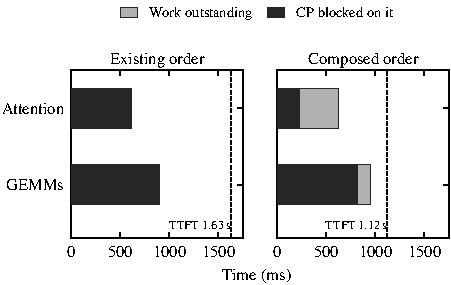
\includegraphics{fig/outstanding.pdf}
    \caption{Per column group, how long the CP was blocked on that group's synchronizations and how long that group's work was outstanding, on a 4{,}096-token prefill of Llama-3.2-1B, from the CP's own record timers. The alternated baseline is the existing program with attention's columns alternated by hand. In it the two quantities are equal for both groups, so the CP was blocked for as long as either group had work and the groups took turns; in the composed order attention's work is outstanding for 626\,ms while the CP blocks on it for 225.}
    \label{fig:outstanding}
\end{figure}
% DECISION: the figure is Llama-3.2-1B only. Qwen3-4B faulted at the driver's debug-buffer sync on teardown in both runs that enabled the records, at two buffer sizes, and wrote none (decisions log D15); its gates still hold (logits identical, TTFT within 0.5%). Absolute times are quoted at 1,800 MHz; a queue-robust fit of the same records gives 1,864-1,941 MHz, so the millisecond values carry 4-8% of scale uncertainty, which does not affect the ratios between arms.

\subsection{The Captured Prefill of the Closed Stack}
\label{app:capture}

% VALUE: under the route attribution, the one captured FastFlowLM prefill changes group only between commands, so it issues serially, one group per command; serial issue predicts its time where overlap does not; a column census agrees without establishing it; MLIR-AIR's fused prefill shares the placement, so its removals bear on the same column groups
% [Note: the first sentence is the clause "either with a recording library that never opens the device or with an interposer during a device run" of the body's closed-binaries sentence, given its own subject and verb; the second sentence's opening names the rule of Section~\ref{subsec:closed}, where the original said "Under this attribution"; "Appendix~A" in the original is written as its label; "Its decoded configuration" is written "The decoded configuration of MLIR-AIR's fused prefill" because its antecedent stays in the body.]
We record FastFlowLM's streams either with a recording library that never opens the device or with an interposer during a device run.
Under the attribution by routes of Section~\ref{subsec:closed}, the one capture we analyse, a 1{,}009-token prefill of Gemma-4-E2B, changes column group only at the boundary between two commands, once into attention and once out of it in every layer, so it issues serially, one group per command.
The sum of its commands' times measured alone, each less the dispatch floor and plus the boundary cost between commands, matches its measured time within 10.0\%, whereas full overlap would place it 36.5\% lower, a separation far wider than the batch-to-batch variation of the read cap this machine shows.
A census of which columns carry any instruction, over all 218 recorded streams and over the capture itself, agrees with this attribution without establishing it, since it counts addressed columns rather than the programs they serve; Appendix~\ref{app:attribution} gives the counts.
The decoded configuration of MLIR-AIR's fused prefill places the GEMMs on columns 1--6 and attention on columns 0 and 7, as FastFlowLM's fused prefill does, so the two share the column groups whose turns our passes remove.
Appendix~\ref{app:attribution} states how the attribution was chosen, and what the rule registered before it labels the same capture.
% SOURCE: device capture through an XRT interposer, gemma4e-flash:e2b, 1,009 tokens; route maps from the frozen cdo_routes decoder: shim 3 and shim 6 MM2S0 reach only columns 0 and 7; 70 group transitions, all between commands (35 GEMM -> attention, 35 attention -> GEMM) (vault lab-flm-streams (11), (13)).
% SOURCE: ops-per-column census over the 218 FLM streams, recomputed here from the committed artifact (aie-cosched 0400fc9 passes/results/bprime/column_ops.json, from bprime_column_ops.py 879bf80; parsed by aie-cosched-pass-0, counts re-derived independently in this workspace): column sets {1,2,3,4,5,6} 200, {0,3} 8, {6,7} 8, {} 1, all eight 1. Every {0,3} stream carries the bulk of its ops on column 0 (e.g. 1,420 against 384) and every {6,7} on column 7, which matches the frozen route map above (shim 3 and shim 6 MM2S0 reach only columns 0 and 7), so the 16 are attention commands plus their feeding shim. The peer's first message said 192 of 218 and corrected it to 200; 192 is the count among proposal streams only. The one empty stream (186fd90831c87d8c) was earlier reported as "not analysed: one column" and in fact has no ops.
% SOURCE: closed-stack check: T = 1.444 s, serial prediction 1.300 s (error 0.100), overlap prediction 0.917 s (error 0.365), tolerance 0.2075, of which 0.102 is one slow floor repetition; without it the tolerance is 0.106 and the serial prediction still passes (vault lab-flm-streams (12) RESULT, amd-npu 52c8401d, 3d0d1036).
% SOURCE: MLIR-AIR's llms README: "reimplement AMD NPU LLM designs originally developed by the FastFlowLM team" (mlir-air 740cae0f, a3e26261); fused_prefill/device.py "laid out like FastFlowLM's fused_prefill"; FastFlowLM's Gemma4-E2B fused_prefill.xclbin decoded with tools/xclbin_layout.py: attention programs on columns 0 and 7, a GEMM program on the 24 cores of columns 1-6 (vault lab-flm-streams (5)); coverage ruling D13(b).
% DECISION: the serial label is scoped to this one capture (Gemma-4-E2B, 1,009 tokens, the engine's cap); the attribution by routes was ruled after the capture, and the label under the first attribution by tile column was MIXED-majority; both disclosures go to the appendix (outline v9 section 2, C2).

\subsection{Further Instances on the Grid}
\label{app:grid-more}

% VALUE: detail behind Table grid's cells that the body does not need: the pair-level order dependence a hand edit created in its unrolled decode loop; the stream name dependences on the fused decode's next-launch writes; per-chunk naming makes the prefill's rings add nothing beyond reordering; the census covers IRON and the production engine, which the table does not
% [Note: the first sentence is verbatim; the second is the clause "and, in the fused decode, on the next launch's runtime-parameter and lock writes" of the body's stream name-dependence sentence, given its own subject and verb; the third is the body's ring clause made a sentence (Section~\ref{subsec:rings} states the same, so the consolidator may drop it here); the fourth is verbatim, with "this table" written as its label.]
Acquires that cover a pair of blocks, the order dependence a hand edit created, arose only in that edit's unrolled loop.
In the fused decode, name dependences in the stream also fall on the next launch's runtime-parameter and lock writes.
The existing prefill already gives each chunk its own data buffers, so rings add nothing beyond reordering, within 0.1\%.
The census extends the same reading to IRON and to the production engine's streams, which no instance in Table~\ref{tab:grid} covers (Section~\ref{subsec:census}).
% SOURCE: the pair-level order edge of the hand edit's arms (b) and (c) came from the pair unroll (lab-cosched-passes (30), item 5; outline v9 section 1); configuration writes as NAME edges on the fused decode only (7,244) (aie-cosched 93f491b, mlir-aie f9ad95dc02f, lab-cosched-passes (62), P7c).
% SOURCE: rings beyond reorder in the stream: R-ship = pair within 0.1% (amd-npu 71081d1).

\section{Pricing Details}
\label{app:pricing-details}

\subsection{DRAM Read Rates by Regime}
\label{app:dram-regimes}

% VALUE: the pair measurements that give the two overlap regimes, in absolute read rates against the cap, and the per-command read rates of a whole prefill that place the GEMMs near the cap and attention far below it; the composed order lowers the GEMM group's rate in the direction the penalty predicts
We measure the overlap regimes of Section~\ref{subsec:removal} on pairs of one attention operator and one GEMM, issued in one command on disjoint columns.
Where the GEMM holds the critical path, on four pairs (five runs) reading 42.9--52.3~GB/s against a measured cap of 53.9--55.3~GB/s, co-running costs it 8.4--10.5\% of the attention operator's device time.
Where attention holds the critical path, co-running costs at most 15~$\mu$s on the five pairs we measure and does not grow with the GEMM's duration.
Per-command read rates during a whole prefill identify the two regimes directly: on Llama-3.2-1B at 4{,}096 tokens, commands that carry only GEMMs read 50.0~GB/s at the median, which is 90--93\% of the cap, whereas commands that carry only attention read 8.3~GB/s, about 15\% of it.
Commands that carry both read 48.0~GB/s, so the GEMM remains the operator near the cap.
Between the existing order and the composed one, the GEMM group's rate over the time its work is outstanding falls from 48.6 to 45.6~GB/s, with the five repetitions of each fully separated, which is the direction the penalty predicts at one cell of one model rather than a second estimate of its size.
% SOURCE: per-command read rates from the ML Timeline records, Llama-3.2-1B scratch 4,096, bytes from the TXN BD chains (amd-npu 71901c50 metrics/retro-2026-10-21/dram-retro.txt, verified from the bare): shipped+Ar GEMM-only n = 12,855 commands p10 41.3 median 50.0 p90 52.8 GB/s; shipped+Ar attention-only n = 2,560 p10 8.2 median 8.3 p90 8.8; composer both groups n = 2,560 p10 35.0 median 48.0 p90 52.4; composer GEMM-only n = 1,230 median 47.8; over each group's outstanding time, G 48.6 (shipped+Ar) vs 45.6 (composer) and A 8.3 vs 8.2, per-rep ranges 48.57-48.59 against 45.54-45.62 and 8.32-8.33 against 8.20, fully separated; read cap 53.9-55.3 GB/s (vault lab-metric-fields (1) and its amendment 1).
% DECISION: the per-command rates identify the regimes and the G drop is reported as the penalty's direction only, scoped to one cell of one model, at npu-gap's request; the penalty's magnitude stays the pair-table fit.
% SOURCE: computed in aie-cosched-paper-0 tmp/regime/{pairs,model,final}.py from lab-prefill-overlap (3)'s pre-registered pair table (10 pair-runs on Llama-3.2-1B, 5 attention chunk indices x 3 GEMM shapes, medians of 20, DRAM measured during each concurrent run, cap 53.9-55.3 GB/s): with the GEMM on the critical path the penalty is 3 us + 0.085 x the co-runner's duration (R2 = 0.993, 5 runs, ratio 0.084-0.105); with attention on it the penalty is 21 us - 0.015 x the co-runner (R2 = 0.896, 5 runs, ratio -0.002 to 0.029); penalty against the pair's total DRAM rate correlates at only r = 0.54, so the regime of the critical-path operator is the predictor and total bandwidth is not (vault decisions log, "Regime analysis, step 1").


\subsection{Pricing Derivations}
\label{app:pricing-derivations}

\textbf{Overlap Ceiling.}
% VALUE: the 1.81-1.84x ceiling follows from the measured penalty: two equal operators in sequence take twice one, together one plus the penalty
Two operators of equal duration $d$ take $2d$ in sequence.
Run together with the GEMM on the critical path, they take $d(1 + r)$ plus a fixed few microseconds, where $r$ is the penalty's share of the co-runner's duration, so the gain is at most $2 / (1 + r)$.
Over the measured shares $r = 0.084$--$0.105$, this is $1.84$--$1.81\times$, whereas with attention on the critical path the penalty does not grow with the co-runner, and the gain approaches $2.00\times$ as $d$ grows.
% SOURCE: the pair-table fit of Appendix~\ref{app:dram-regimes}: 3 us + 0.085 x the co-runner, per-pair ratio 0.084-0.105; 2 / 1.084 = 1.845, 2 / 1.105 = 1.810.

\textbf{Granularity of the Test.}
% VALUE: which test applies follows from the grid's granularity; both give the same necessary condition; the ordering case adds typed resources, of which only the group is private
Which test applies therefore follows from the granularity of Table~\ref{tab:grid}: the longest path within a command, and the maximum cycle mean inside an engine's loop.
Both give the same necessary condition on a set $S$ of removals: unless $S$ cuts every path or cycle that attains the maximum, one of them survives with its length unchanged, so the phase is still bounded by it and $S$ gains nothing.
The condition is necessary and not sufficient, for two reasons that this machine supplies.
After a cut, the next longest path or cycle bounds what remains, so the gain is what separates them rather than the whole of $O(S)$.
And the groups share capacity, the DRAM read cap and the shim tiles' channels, so a set that does cut every critical path gains only what that capacity leaves: Llama-3.1-8B's decode already reads its cache at the rate two shim tiles sustain, so renaming every buffer on its loop's cycle hides only the serialized compute (Section~\ref{subsec:decode-eval}).
We therefore use the condition as a test of which candidate sets cannot pay, and leave the magnitude to the event model of Section~\ref{subsec:pricing}.
What the ordering case adds is the typed resources: a removal frees work onto a column group, onto the CP, or onto a DRAM read rate that every group shares, and only the first of those is private, so the share of a phase a removal can recover is not read off the program's order alone.

\textbf{Loss at Short Appends.}
% VALUE: the bound cannot predict a loss; at 512-token appends the composed prefill loses to the existing order because its in-flight pipeline is mostly fill and drain, which the event model prices
At 512-token appends, for example, the composed prefill runs at 0.88--0.93$\times$ the speed of the existing order, which the event model attributes to the composed schedule's per-command costs: with four chunks per layer its pipeline of in-flight commands is mostly fill and drain, so its overlap has little to hide.
% SOURCE: vault lab-agent-step (11) and its reading at line ~602 ("With 4 chunks per layer, the composer's D-deep pipeline is mostly fill and drain. Its overlap has little to hide, and its per-command costs stay"). Corrected 2026-10-22 (D19 convergence point 6): the earlier text named planning, which is outside the timed call.

\textbf{Decode Terms.}
% VALUE: decode's time per token follows a two-term model from measured terms: a fixed part and a per-position cost that is the transfer and the compute in series when the KV loop is single-buffered, and the larger of the two when it is double-buffered; the same model bounds what placement can add
Decode needs a simpler model, because it runs one command per token whose CP order already issues the next weights before it waits on the KV cache (Section~\ref{subsec:losses}).
Its time per token is $T_0 + c\,L$ for a context of $L$ positions, where the fixed part $T_0$ covers the weight reads and the per-position cost $c$ covers attention.
With a single-buffered KV loop, $c = B + C$ for a transfer time $B$ and a compute time $C$ per position, whereas a double-buffered loop gives $c = \max(B, C)$.
Both $B$ and $C$ are measured, $B$ by streaming further positions with no further compute and $C$ as the remainder, and $B$ can fall no lower than the DRAM read cap allows.
% SOURCE: T0 = 15.94 ms, c = 1.156 us (Llama-3.2-1B); B = 0.677 us at the two-shim rate, C = 0.478 us; the cap gives B >= 0.596 us (vault lab-decode-long-context (5), (7)).
% DECISION: the per-model terms for the other models come from the same two probes per model (vault paper-cosched-plan).


\subsection{Partial Renaming of Decode Attention}
\label{app:partial-rename}

% VALUE: decode attention: renaming keys and values alone measured null while the shared score buffer remained, and renaming all three brought each position close to its transfer alone; the critical-cycle reading is an explanation stated before the null arm ran and supported by the per-block fix's bands, not a prediction; the cycle model does not reproduce the existing loop's cost in sample, so its joint prediction was not counted; a one-change-at-a-time search could stop after the first rename; reordering decode's stream can gain little
Decode attention shows the condition at work.
Renaming its keys and values alone, with the score buffer still shared, leaves the time per token within 0.3\% of the existing design's at 16{,}384 and 32{,}512 tokens, whereas renaming all three lowers it by 1.27$\times$ and 1.39$\times$, and each position then costs within 1\% of its transfer alone.
Our reading is that the shared score buffer keeps the two cores waiting on each other and so keeps the loop's critical cycle.
This reading was stated as the explanation of a null result before a hand edit that renamed all three buffers, but acquired the scores once per pair of blocks, measured null, and a per-block score channel then reached gains inside the bands stated before its run.
It explains these results in sample rather than predicting them, and the per-block channel also adds a transfer hop and keeps a coupling per pair of blocks.
% COMMENT (development, D21 revised 2026-10-22): the cycle model's form is being corrected to reproduce the measured 1.15 us per position (the frozen form gave 1.40) and is re-registered for the final sweep; the earlier sentence reporting that development miss is withdrawn per the author's rule that development-phase misses are not disclosed.
Consequently, a search that applies one change at a time and keeps only the changes that help could stop after the first rename.
By contrast, reordering decode's stream could gain at most about 1.13$\times$, since its phases already read DRAM near the cap.
% SOURCE: keys and values renamed with the existing score buffer kept: 1.002x (16,384) and 1.003x (32,512), tokens and logits bit-identical (vault lab-decode-long-context (28); amd-npu d8f0bd4c, score 5e1017a5); all three renamed (the loop pass): 1.269x / 1.391x, slope 0.683 us against a transfer-only 0.677 us (lab-decode-long-context (22)).
% SOURCE: decode reordering or placement bounded at about 1.13x, phases near the DRAM cap (vault lab-bound-validation (1), from lab-decode-long-context (5)-(7)).
% SOURCE: the explanation stated before arm (b) ran: lab-decode-long-context (11); (c)'s bands 0.68-0.78 us, 1.22-1.29x, 1.30-1.41x, hit at 0.712 us, 1.274x, 1.366x, the gate's +-3% at 2k missed on the good side by 5.1% (lab-decode-long-context (12)-(13)); the cycle model's census gate 1.399 vs 1.153 us per position, tolerance 0.112; J predicted 1.079x / 1.106x, band lower edges 1.0088 / 1.0095, measured 1.0018x / 1.0027x, outcome UNTESTED (cells uncounted) (lab-decode-long-context (27)-(28); amd-npu a3334f8d).
% DECISION: the critical-cycle wording is outline v9's W2 row (the census gate failed): the base wording, the in-sample clause, and J's outcome as a clause; the 1.231 vs 1.153 us diagnosis stays open.

\section{OPCORD Details}
\label{app:opcord}

% VALUE: the parts of OPCORD a reader needs to reproduce it but not to follow Section 6's argument: the composer's plan and issue order in full, the host boundaries, the argument arenas, the rings and their memory, the loop pass's changes to the lowered design, the splits and what switching between them costs, how the checkers are checked, what the platform must offer, and where the work would move into the compiler
This appendix gives the parts of OPCORD (Section~\ref{sec:method}) that a reader needs to reproduce it but not to follow its argument.

\subsection{Issue Order}
\label{app:issue}

% VALUE: the composer's inputs and plan in full: it takes the per-operator streams, the column map, the host program's dependency graph, and the probes; each step pairs the lowest ready attention operator with ready GEMMs in plan order until their estimated work matches; the GEMMs then run in sequence on their columns while attention runs on its own
For the open prefill, the composer takes an existing design's per-operator instruction streams, its map of operators to columns, the dependency graph of its host program, and the probes, and emits a sequence of composed commands.
The composer splits each operator's instruction stream, already reduced to its own columns, into segments.
At each step, it takes the ready attention operator of the lowest layer and chunk and adds ready GEMMs, in the same order, until their estimated work reaches that of the attention operator.
The GEMMs then run in sequence on columns 1--6 while attention runs on columns 0 and 7.
For an append to a cached context, the composer plans only the new chunks, and their attention estimates use each chunk's absolute index.
% SOURCE: merged.plan (amd-npu a0ee2ed, now opcord/compose/merged.py at aie-cosched opcord-runtime 446fa1c): qkv(L, c) after down(L-1, c); attn(L, c) after qkv(L, 0..c); o after attn; gate and up after o; down after gate and up; an optional cap on the GEMMs per attention command.
% SOURCE: append = Merged.prefill(ids, start=L) on the same plan rules; attention estimates linear in the absolute chunk index (vault lab-agent-step (1)).

% VALUE: how predicted completion is computed, and the condition under which the composed order matches the list schedule of the groups without a CP, stated as a remark
A GEMM's synchronizations are predicted to complete after the sum of the estimates of the GEMMs up to and including it, and attention's mid-stream synchronizations at fixed fractions of its estimate.
When issue costs are negligible, the estimates are exact, and the host work is hidden, the CP never blocks on a later-completing operator while an earlier one's successor waits, so the order matches the list schedule of the groups without a CP.
% SOURCE: merged.cp_order (a0ee2ed, now opcord/compose/merged.py); mid-stream fractions (0.25, 0.5) of attention's estimate, the lowest of five placements tried; the in-turn order takes 1.26x as long on the same 38 commands (lab-prefill-overlap (16)).
% DECISION: the exactness statement in the last sentence is argued, not proven; it stays a remark until a proof is written (vault ch3-formulation, Lower bound and heuristic).

% VALUE: the price of running the two groups at once: the columns share the DRAM read cap, so a group whose partner is bandwidth-bound loses a measured share of its partner's time, and the ceiling on a pair is below the ideal; where a group is already near the cap there is nothing to win
Running the two groups at once is not free, because the columns share one DRAM read rate.
A group on the critical path loses 8.5\% of its partner's duration when it is bandwidth-bound and almost nothing when it is not, so two operators of equal duration overlap to within $1.84\times$ of the longer rather than the ideal $2.00\times$ (Section~\ref{subsec:removal}).
Where a design already reads near the cap the reorder therefore has little to recover, which Section~\ref{subsec:bound-eval} reports for the largest model we evaluate.
% SOURCE: the penalty by regime and the 1.84x ceiling are Section 5's measurement; per command on Llama-3.2-1B at 4,096 tokens, commands carrying GEMMs read 90-93% of the cap and commands carrying attention about 15% (vault decisions log, "Regime analysis" steps 1 and 3); the 8B composed prefill averages 93-96% of the cap (lab-metric-fields (1)).

\subsection{Host Boundaries}
\label{app:host}

% VALUE: host work between commands forces boundaries; keeping D commands in flight hides the host work and the boundary cost but delays which operators are ready, so the depth, a cap on GEMMs per attention command, and the packing of GEMMs without attention are chosen per regime with the event model, and reported apart from the essential decisions
Since the host computes normalizations, rotary embeddings, and residuals between commands, a dependence that crosses the host forces a command boundary.
The composer keeps $D$ commands in flight and processes a command's outputs while later commands run, so a command can carry only operators whose inputs come from commands at least $D+1$ positions earlier, unless a step with nothing ready drained the queue between the two, in which case an input may come from the command just before.
% SOURCE: vault lab-split-sweep (35), K-d corrected wording, enforced by a runtime check_posted assert (amd-npu 8073b924, 26/26 composer-check tests green).
A step without a ready attention operator packs a fixed number of ready GEMMs into one command, following standard practice for amortizing dispatch cost (Section~\ref{subsec:semantics}).
The depth, the cap on the GEMMs that join an attention operator, and the packing are chosen per regime together with the split, by the event model (Section~\ref{subsec:split}), and we report their effect apart from that of the essential decisions (Section~\ref{subsec:formulation}).
% SOURCE: opcord/plan/planner.py choose() at aie-cosched opcord-runtime 446fa1c: depth {1, 2, 4, 8} x GEMM cap {none, 4} x packing {1, 4}, priced by the event model with every split (decisions log D24 N3). The evaluation's present cells used amd-npu prefill-overlap/v1/POLICY.md: "Chosen by (18)'s pre-registered rule: the measured-fastest arm per length"; POLICY = {2048: (4, None, 4), 4096: (2, 4, 4)} (D, GEMM cap, packing).
% DECISION: this states the current planner; the earlier sentence (the measured-fastest arm per length) described the composer the present cells were measured with, and the final sweep runs through choose().

% VALUE: the price of depth: it hides the host's work but delays which operators are ready, and what it is worth falls as the prompt grows, so the right depth is a property of the workload rather than of the design
Depth trades the host's exposed time against how early an operator becomes ready, and what it buys falls as the prompt grows.
Without commands in flight the host is exposed for 9.3\% of TTFT at 2{,}048 tokens, against 0.5\% at the composer's depth there and almost none at 4{,}096.
The existing host program instead keeps every command of a stage in flight, 32--64 of them, and so pays no exposed host time and gains no choice of order.
% SOURCE: host-exposure share under the composer's policy 0.5% of TTFT at 2k and about 0 at 4k, against 9.3% without queue depth at 2k; the shipped program keeps 32-64 commands in flight against the composer's 2 (vault lab-prefill-overlap (16) and its pre-registration; lab-split-sweep (18)).
% SOURCE: merged.plan with lag = D; Layout claims an output slot when its command is queued, D - 1.6 commands before it runs (a0ee2ed).

\subsection{Argument Arenas}
\label{app:arenas}

% VALUE: the existing design binds one buffer per argument slot, so a command holds only one GEMM; we retarget only a patch's byte offset, never its slot, so any number of GEMMs share the GEMM slots through arenas, under an offset bound the composer respects; attention needs three slots per group at any split
The existing design gives each operator kind its own argument slots, so a command that carries attention can hold only one GEMM.
Since retargeting a patch to another slot faults in the IOMMU whereas changing its byte offset is safe, we allocate the GEMM inputs, weights, and outputs as sub-buffers of three parent buffers, which we call \emph{arenas}, and rewrite only each GEMM's patch offsets, so any number of GEMMs share three slots.
The offset field bounds an arena to $2^{31}$ bytes, so the weights are split into arenas of whole layers, and the GEMMs of one command share a weight arena.
The composer serves every split with three argument slots per attention group instead of a fixed six.
% SOURCE: nine slots, nargs = 3 + 3 x len(cfg.attn) (mlir-air a3e26261 engine.py:107); address patch = opcode 0x81, argument index at word 8, byte offset at word 10.
% SOURCE: slot moves complete with wrong output and AMD-Vi IO_PAGE_FAULT lines; offset moves inside a parent buffer are bit-identical; two GEMMs at distinct offsets in shared arenas are bit-identical (amd-npu 61c64f9 prefill-overlap/retarget/, lab-prefill-overlap (8)).
% SOURCE: merged.Weights (a0ee2ed); Llama-3.2-1B uses one weight arena, Qwen3-4B two (2145 + 195 MB) (lab-prefill-overlap (24), (26)).

\subsection{Buffer Rings}
\label{app:rings}

% VALUE: how the composer derives its rings: each use lives from its producer's write to its last reader's completion, interval colouring assigns slots, a separate check rejects early reuse, and the depths follow from the plan
For each buffer role, the composer derives a ring of slots from the plan.
Each use of a buffer lives from its producer's write to its last reader's completion, and interval colouring assigns slots so that no two overlapping uses share one.
A separate check asserts, over the whole plan, that no slot is reused before its previous reader has completed.
The depths follow from the plan and are not set by hand; for example, every QKV input of the first layer is written before that layer's first QKV command completes, so that ring needs one slot per chunk.
% SOURCE: merged.colour, assert_no_hazard, and Layout (a0ee2ed); the hazard check turns red on an overlapping slot; ring depths at 4,096 tokens: shared 2048-wide input 32, 8192-wide input 4, outputs 4-18 (lab-prefill-overlap (9)).

% VALUE: the price of the rings: slots are memory, and the composer buys overlap with it; the rings take fewer bytes than per-chunk naming at no change in time; the arenas replace the engine's own weight buffers rather than adding to them, so the cost is the schedule's slots and not a second copy of the weights
Slots are memory, and the rings take 4--7$\times$ fewer bytes than the per-chunk naming they replace, with no change in time, within 0.1\%.
The rings and the plan's own buffers take 53--179\,MB across the configurations we build, whereas the arenas that hold the weights replace the engine's own weight buffers rather than adding to them, so the weights are not copied twice.
Peak live device memory for a 4{,}096-token append to a 16{,}384-token context is then 3.5\,GB on Llama-3.2-1B, 7.7\,GB on Qwen3-4B, and 9.7\,GB on Llama-3.1-8B; the production engine holds 2.2 and 7.9\,GB for the first two on the same weights, so the schedule's slots and not a second copy of the weights are what we add.
% SOURCE: shipped naming is one slot per role per chunk; R-ship (the composed schedule at shipped's per-chunk naming) equals the composer with rings within 0.1% (0.99996-1.00074, amd-npu 71081d1) and holds 4-7x the rings' buffer bytes (vault lab-prefill-overlap (29), third revision).
% SOURCE: composer schedule buffers (Layout plus lazy) 53.4-178.8 MB over the 21 configurations (min 1B S4 16k + 4k, max 8B S2 scratch 2k; amd-npu 71901c50 metrics/retro-2026-10-21/footprint-summary.txt, re-derived in the 2026-10-22 foundation audit); weight arenas 645 MB (1B), 2,340 (Qwen3-4B), 4,451 (8B), replacing rather than duplicating the engine's weight buffers, with peak minus live equal to the arena size within 2% at load; peak live 2,206 / 5,923 / 7,399 MB at 4,096 tokens from scratch and 3,471 / 7,725 / 9,721 MB at 16,384 + 4,096; FastFlowLM's server at drm-total-memory 2,110,100 KiB (1B) and 7,668,316 KiB (Qwen3-4B), i.e. 2.16 and 7.85 GB (mapped 2,158,084,096 and 7,847,751,680 B; the earlier 2.11 / 7.67 read KiB as kB) (vault lab-metric-fields (1); lab-flm-practice (3)).
% DECISION: the tradeoffs are stated beside the decision that incurs them rather than collected in a section (author, 2026-10-21).

\subsection{The Loop Pass}
\label{app:loop-pass}

% VALUE: why the ring is acquired once per block on both ends: renaming all three buffers while acquiring the scores once per pair of blocks, as a hand edit unrolled by two does, leaves the time per token within 2% of the existing design's, because the two cores still wait for each other; the pass matches a hand edit with a score channel within 1%
Renaming alone is not enough, however, when the scores are acquired once per pair of blocks, as in a hand edit that unrolls the loop by two.
With the keys, values, and scores renamed but the scores acquired per pair, the time per token stays within 2\% of the existing design's, since the core that computes a block's scores and the core that folds them into the output still wait for each other.
On both models, the pass's output comes within 1\% of a hand edit that passes the scores between the cores through a channel instead, at every evaluated length.
% SOURCE: renamed K, V, and score in the hand edit unrolled by two, scores acquired per pair (arm (b)): 0.997-0.984x per token at 4k-32.5k, slope 1.181 vs 1.153 us (Llama-3.2-1B; vault lab-decode-long-context (13), amd-npu aab2aae); the same edit on Llama-3.1-8B 0.990x at both cells (lab-decode-long-context, decode nulls Phase 2). Loop pass (aie-cosched-rename, mlir-aie 41b4947f09e; classes and rings in vault lab-cosched-passes (33)): against the existing design 1.269x at 16,384 and 1.391x at 32,512 (1B), 1.160x at 16,384 and 1.205x at 28,800 (Qwen3-4B); pass / hand edit 0.992-1.004 at every point; slope 0.683 us (1B) against a transfer-only 0.677 us; tokens and every step's logits bit-identical across the existing design, the hand edit, and the pass, 1B P = 0 to 32,517 and Qwen3-4B P = 2,048 to 28,800 (vault lab-decode-long-context (22), amd-npu a6bc94b and 455740b).
% DECISION: the rename is our loop pass's output on the lowered design, not a hand edit; the hand edit appears only as the reference the pass reproduces.

% VALUE: what our loop pass changes in the lowered decode design, in local memory and in the configuration, what it skips and why, and that it keeps one kernel call per block and leaves every build output unchanged when switched off
The pass gives each renamed buffer a twin on the same tile, raises its free-slot lock from one slot to two, extends its buffer-descriptor chain through the twin, and selects the slot in each iteration through a one-word rotation counter in local memory that the configuration initializes.
It keeps one kernel call per block, so the loop runs exactly the blocks that the context needs, and it lists with a reason, rather than renames, any buffer whose synchronization is not one lock pair or whose twin would exceed the tile's 16 buffer descriptors or 64\,KiB of local memory.
The pass runs as an opt-in step inside the existing compiler, and with it switched off, every instruction stream and configuration that the compiler emits is byte-identical to the existing build.
% SOURCE: aie-cosched-rename, mlir-aie 41b4947f09e: 12 buffers renamed on the 1B census build (K, V, score per attention pair), 0 over budget, 16 / 16 rotation words written by the PDI's initial-value writes (vault lab-cosched-passes (33)); hook-off identity PASS on the 1B and Qwen3-4B, differences confined to xclbin / PDI UUIDs and timestamps, as between two stock builds (vault lab-decode-long-context (20)-(22), control 2).

\subsection{Splits and Their Costs}
\label{app:relayout}

% VALUE: how the existing design encodes the split, how each split is built and checked, and how the composer predicts per split
The existing design fixes the split of columns between attention and the GEMMs by hand: attention groups are listed per column, and the GEMMs take a contiguous block of the remaining columns.
A model with 8 KV heads admits attention on 1, 2, or 4 columns, with the GEMMs on the other 7, 6, or 4.
We build each split as its own configuration from the unchanged design source, which takes seconds.
The composer checks every GEMM's encoded iteration count and stride against the shim BD's field limits before it uses a split.
For each split, the composer probes every operator alone once and predicts the TTFT of each regime with the event model (Section~\ref{subsec:pricing}).
% SOURCE: mlir-air a3e26261 fused_prefill/device.py: Attn(col=...) per group in Config.attn, GCOL0, GNC = 1, 6 as module constants; spec() splits kv_heads evenly, so 1, 2, or 4 attention columns with 8 KV heads (vault lab-split-sweep (1)).
% SOURCE: out-of-tree split modules, builds of 13-14 s; logits bit-identical to the default split in every configuration on both models (vault lab-split-sweep (2), (4), (5)).
% SOURCE: BD iteration wrap 6 bits (at most 64 rounds), stride 20 bits (words); the four-column split's LM-head GEMM runs 48 rounds; decoded from aie-rt xaie2pgbl_params.h fields with a round-trip check (vault lab-split-sweep (5)).
% SOURCE: per-split probes at n = 2,048, prediction with component_model.simulate (amd-npu 0f61651 prefill-overlap/g1_split_model.py, vault lab-split-sweep (6)-(7)); now event_model.predict through choose() (aie-cosched opcord-runtime 446fa1c).

% VALUE: the price of making the partition a per-regime choice: each split is its own configuration, so a deployment either holds two of them with two copies of the weights or pays a switch and a cache relayout; the weights are the larger of the two costs on a large model
Making the partition a choice therefore costs either memory or a switch.
Each split is its own configuration, so holding both resident holds the weights twice, which on Llama-3.1-8B is 4.5\,GB of weight arenas for each; releasing one instead costs a warm switch, 7--8\ms{} on the two smaller models, and a relayout of the cached context.
Neither cost applies within one regime, where a single split serves every turn.
% SOURCE: weight arenas 645 MB (Llama-3.2-1B), 2,340 (Qwen3-4B), 4,451 (Llama-3.1-8B), one copy per resident split (vault lab-metric-fields (1)); warm switch 7.1 ms (1B) and 7.7 ms (Qwen3-4B), suspend and resume only, without moving a cached context (lab-split-sweep (5)).
% SOURCE: switch = suspend + resume + first prefill in one process, both splits' weights resident (vault lab-split-sweep (5)).

% VALUE: the relayout measured: linear in the bytes moved, mostly the host's encoding of the block format, bit-identical; it costs 3.5 to about 120 times the warm switch, so frequent switching favours holding both splits and a single switch favours moving the cache
Moving the cached context between splits is the cost that decides between the two paths.
Re-encoding the cache's per-block records for the other split's attention groups takes 25, 112 and 203\,ms on Llama-3.2-1B and 106--108, 487--499 and 874--892\,ms on Qwen3-4B for cached contexts of 4{,}096, 16{,}384 and 28{,}672 tokens, linear in the bytes moved at 392 and 381\,ms per GB, and every moved record and the next append are bit-identical to the target split's own prefill.
Most of it is the host's encoding of the block format, 72--76\% of each move.
A move therefore costs 3.5 to about 120 times the warm switch, so a deployment that switches regimes often holds both splits resident and pays the memory instead, whereas one that switches once in a session pays between a fortieth of a second and under one second.
% SOURCE: amd-npu d159d53f prefill-overlap/relayout-run2-2026-10-22/score.json (relayout_score.py at 6d251fc5, unchanged; outputs 75267405 committed before reading), medians of 5 per cell, both directions S2<->S4: 1B 24.7 / 25.0, 112.8 / 112.3, 202.8 / 202.3 ms; Qwen3-4B 107.6 / 105.9, 498.8 / 487.5, 892.0 / 873.5 ms; slope 392.2 / 380.7 ms per GB, max residual 2.3 / 1.4%; every records and append gate bit-identical (vault lab-split-sweep (38)); verified from the bare by aie-cosched-c8. Phase shares: encode 72-76%, host K/V concat 18-22%, sync 4-7%. Ratios use the 7.1 / 7.7 ms warm switch (lab-split-sweep (5)).

\subsection{Checker Agreement}
\label{app:checkers}

% VALUE: each checker is checked against a second, independent implementation that derives its facts by another route; the stream checkers agree on every verdict over every prefill build and the 42 hand-alternated streams, and refuse ten negative controls with identical reasons; every rename the loop pass refuses, forced, yields a design the second implementation refuses; without forcing, the pass renames nothing there and its output is accepted
Each checker inside a pass has a second implementation, written separately, that derives its facts by another route; for the stream checker, the pass reads the routes from the device's IR, whereas the second implementation decodes them from the configuration binary.
On every prefill build we hold, the two derive the same facts for 110 operators, and on Gemma3-4B's builds they differ only where the second implementation cannot resolve a lock's acquire from the compiled core program and reports so, which no verdict depends on.
They agree on every verdict, including all 42 hand-alternated attention streams, where the pass's rewrite is byte-identical to the hand version, and both refuse ten negative controls with identical reasons.
For the loop pass, the second implementation interprets the original and the renamed design, and it refuses a rename whose reads differ from the original's, that deadlocks, or that races.
Forcing the loop pass to rename one buffer of each class it refuses on the decodes, through an option that exists only for this test, yields a design that the second implementation refuses in every case, because its reads differ from the original's.
Without the option, the pass renames nothing in those inputs, and the second implementation accepts its output.
% SOURCE: P6 (decisions log, "P6 steps 1-5 done"; vault lab-cosched-passes (57) steps 3-5): route facts R1 (C++ from the device IR) against the Python oracle (from the CDO); 0 differing facts on 110 operators (1B S4, in-tree, S1; 8B S4, in-tree; LFM2 S4, in-tree, S1; Qwen3-4B S1); Gemma3 S4 86 and in-tree 41 per operator, all the oracle's TOOL-FAILED condition (4), counted apart, and no verdict met one; every moved stream AGREE, 0 DISAGREE; the 42 hand-alternated streams 162 / 162 AGREE (30 linear variants each checked against all five candidate operators), the C++ rewrite's bytes equal to the hand versions; 10 negative controls AGREE with identical codes; mlir-aie cosched-flag e20940fac7e.
% SOURCE: forced refusals (lab-cosched-passes (57), "The loop pass's refusals, confirmed by forcing": mlir-aie aie-cosched-pass-0 7669b8d4e7b, cosched-flag e20940fac7e; aie-cosched b36c5d2, results/2026-10-23-rename-force/): classes (a) unsupported nested control, (b) used outside a block loop, (c) free-slot lock not starting at 1, (d) not one free / full lock pair, each forced and REFUSED by loopcheck with READS-DIFFER; negative controls without force= rename nothing and are accepted; loopcheck outcomes READS-DIFFER, DEADLOCK, RENAME-INEFFECTIVE, WORD-UNINITIALIZED, UNSUPPORTED, RACE.
% DECISION: the oracle's RACE on the shipped decode's core 2_2 (buf154) is not stated here; reporting it is the author's call (decisions log, P6).

\subsection{Platform Requirements}
\label{app:platform-req}

% VALUE: what a platform must offer for OPCORD to apply: an in-order issuer whose issue returns at once and whose waits block, disjoint groups that share only DRAM, per-operator streams, and buffers named by slot and offset
The composer relies on four properties of the platform rather than on MLIR-AIR: a single in-order issuer whose issue instructions return at once and whose synchronizations block, column groups that share only DRAM bandwidth, a design whose operators expose their own instruction streams, and buffers that commands name by an argument slot and a byte offset.
% SOURCE: Sections 2.1 and 3.1; the five q4nx models of the evaluation all run on AIR's shared fused prefill and fused decode (mlir-air a3e26261 programming_examples/llms/*_q4nx).

\subsection{Moving into the Compiler}
\label{app:compiler}

% VALUE: answers the obvious question of why one of the three passes runs on the host while the other two are compiler passes. The answer is a condition rather than a boundary: the two inside the compiler are the two whose output does not depend on the prompt, and a deployment whose shapes are known could emit the composed stream ahead of the run as well.
Where this work would move into the compiler is decided by when the shapes are known.
Two of our three passes already run there, and they are exactly the two whose output does not depend on the prompt: the stream pass reorders the segments within one operator's stream, and the loop pass renames the buffers of decode attention, and one build of each serves every context length.
The composer is the piece that runs at dispatch, and it is the piece whose plan is a function of the cached context and the appended tokens.
Nothing in that plan requires a host.
Planning a schedule and composing its commands are compile-time work in kind (Section~\ref{subsec:setup}), and a compiler given the shapes could emit the composed stream before the run, at the cost of one plan per shape rather than one build per shape.
A deployment whose shapes are fixed therefore needs no dispatch-time planner, however large those shapes are, which is what a fixed chunk size secures~\citep{xu2025llmnpu}.
An agent appends whatever its tools return to a context that grows each turn, so its shapes belong to the turn rather than to the deployment, and planning each one in a fraction of a second is what avoids enumerating them in advance.
% SOURCE: the split builds are per configuration and not per shape, 13-14 s from unchanged source (Appendix~\ref{app:relayout}); planning and composing are per shape, 63-206 ms and 56-148 ms on Llama-3.2-1B and 0.3-1.1 s and 143-368 ms on Qwen3-4B (Section~\ref{subsec:setup}); the decode design is one build per 32,768-token window, with the position setting trip counts at runtime (figs/data/decode-1b.json, windows 32768).
% DECISION: stated as a condition, not a boundary, and the compiler claim is argued rather than demonstrated: no pass in our trees composes across operators, so the sentence says "could" and names no gain.

\section{Evaluation Details}
\label{app:eval-details}

% writerG-appendix.tex: material relocated from 7-eval.tex by the evaluation rewrite (writerG-eval.tex).
% Each block names where it goes in appendix-body.tex. Text is verbatim from 7-eval.tex at 548aa83 unless a
% "% EDITED:" line says otherwise; references to section numbers are replaced by \ref where the label exists.
% New labels: app:setup, app:overheads, app:handoff, app:percell, app:census. Existing labels extended:
% app:flm, app:synthetic, app:gemma-gate, app:flags, subsec:tests.

% ======================================================================================================
% NEW SECTION, after app:roundtrip (or wherever the author places setup material)
% ======================================================================================================
\subsection{Evaluation Setup in Full}
\label{app:setup}

% VALUE: the setup's detail that the body states in short form: the three append grids and which result uses each, how the stronger baseline is built, how each batch is controlled, and how the reference to FastFlowLM is bracketed
\textbf{Workload Grids.}
% EDITED: the leading clause "Prompts computed from scratch have 2,048 or 4,096 tokens." stays in the body.
Appends to a cached context come in three grids: 4{,}096 tokens onto 4{,}096 or 16{,}384 for the comparison of schedules (Section~\ref{subsec:ablation}); 4{,}096 tokens onto 2{,}048 or 8{,}192 and 2{,}048 onto 12{,}288 for the absolute times, the model's accuracy, and the bound (Table~\ref{tab:append}, Section~\ref{subsec:accuracy}); and 512, 1{,}024, or 4{,}096 tokens onto 4{,}096, 16{,}384, or 28{,}672, followed by 250 generated tokens, for an agent's turn.
These appends range from below the median to below the 90th percentile of the new tokens per step in coding-agent traces~\citep{zhu2026tracelab}, whereas the contexts stop at the 32{,}768-token window of the decode designs we build, below the traces' median prefix of 119K tokens.
% SOURCE: TraceLab Table 8: append tokens P25 / P50 / P90 = 384 / 857 / 5,342 (Claude) and 406 / 886 / 8,310 (Codex); output P50 252 / 184; Section 1: median prefix 119K, append 875, output 214 (PDF read 2026-10-15).
% SOURCE: turn cells excluded before running: 28,672 + 4,096 (L + N + 250 > 32,768, the 1B decode window); Qwen3-4B at 28,672 (its decode KV buffer passes the 4 GiB shim-offset bound) (vault lab-agent-step (5)).
% DECISION: the grids are named where each registered number is quoted, per the design review: the tolerance and the bound's range were scored on appends of 4,096 or 2,048 tokens onto cached contexts of 2,048, 8,192 and 12,288, whereas the turn results are measured on contexts of 4,096, 16,384 and 28,672 with appends of 512 to 4,096. The two grids are disjoint, and no turn cell carries a scored prediction.

\textbf{The Stronger Baseline.}
The baselines are each design's own host program on its default split and, as a stronger baseline, the same program after we apply by hand the optimization an expert would reach for first: alternating the segments of attention's two columns so that both start before either is awaited. We construct that arm ourselves; no stack ships it. It uses the same configuration, kernels, and weights as our schedules, and it removes the one false dependence that is visible without reading the command stream, so the gains we report are over a program that already has had the obvious fix; FastFlowLM~\citep{fastflowlm-repo} on the same weights gives an absolute reference.

\textbf{Batch Control.}
Each batch of runs holds the device exclusively, checks that no other process has it open, and brackets the runs with a DRAM bandwidth probe and an empty-command dispatch.
Because the aggregate DRAM read cap varies by up to 12\% between batches, every ratio between our schedules compares runs within one batch; the reference to FastFlowLM compares batches taken on different days, each bracketed by its own probe.
We report the median of five timed runs of prefill and three of decode and turns after one warm run (five, paired, for Llama-3.1-8B's decode), with the order of schedules rotated between rounds.
TTFT is the wall time of the prefill call, from token identifiers to logits, decode time per token is measured over 250 greedy tokens after a prefill of the context (256 on Llama-3.1-8B), and a turn's time is its append and its 250 decoded tokens.
% SOURCE: lock = flock ~/.local/state/npu.lock; brackets = 1x1 and 8x2 DRAM reads of 256 MiB, the dispatch floor, load, NPU mode, EPP, governor; 8x2 cap 49.9-55.7 GB/s over the batches, 55.7 / 49.9 = 1.116 (lab-prefill-device (1), lab-prefill-overlap (2), (11), lab-split-sweep (4)-(5), lab-agent-step (2)).

% ======================================================================================================
% INTO app:gemma-gate, as its opening paragraph (before "Three kinds of instrument ...")
% ======================================================================================================
% VALUE: the body's gate sentence in full: what the gates compare against, the 1B result that clears the turn model's prefill path, the Gemma3-4B divergence and why its prefill times still stand
Every run's logits must be bit-identical to the baseline's, every append's logits bit-identical to those of a full prefill of the whole prompt, and the kernel log must show no driver or IOMMU message during the run.
These gates compare a schedule with the stack's own output rather than with an independent implementation of the model, and where a stack also supplies a floating-point forward we compare against that.
On Llama-3.2-1B, which carries our decode and turn results, the prefill's keys and values differ from that forward by up to 3.0\% and 7.5\% across layers, yet decode seeded from the forward's own keys and values, from one split's, and from the other's emits the same seventeen tokens.
On Gemma3-4B the same comparison diverges at the fifth decoded token and we report no turn for that model; the difference is the shipped program's own, since a build made by the module's own builder and loaded by the module's own path produces, bit for bit, the keys and values our harness hands to decode.
We still report that model's times, because under the static control of Section~\ref{subsec:model} a dispatch's work is fixed by its runtime parameters rather than by the values it computes, so the schedule's duration does not depend on the arithmetic the shipped program produces; what the comparison bears on is that program's accuracy, not our measurement of it.
% EDITED: the body's pointer "Appendix~F gives both comparisons and the per-layer differences." is dropped here, since this paragraph now opens that appendix.

% ======================================================================================================
% NEW SECTION: composition and planning cost (the body's Overheads cites it)
% ======================================================================================================
\subsection{Composition and Planning Cost}
\label{app:overheads}

% VALUE: why planning and composing are not inside the measured call, with the existing program's equivalent measured, and the per-request charge that bounds the worst case
Planning a schedule and composing its commands are compile-time work.
The shipped program's instruction streams are emitted by its compiler before any prompt runs and are no more inside its measured call than ours are inside the composed one: timing the shipped arm's first call against its later ones puts its own per-call composition between $-80$ and $+87$\,ms.
Our composer does the equivalent work when a prompt shape is first seen, and keeps it: on the two-column split, composing a shape's commands costs 56--148\,ms on Llama-3.2-1B and 143--368\,ms on Qwen3-4B, and planning it 63--206\,ms and 0.3--1.1\,s.
Even charged on every request rather than once per shape, the composed schedule on that split stays ahead of the shipped program at every cell we measure, by $1.18$--$2.18\times$ and $1.13$--$1.53\times$.
A small part of this work is inside the measured call already, 7--14\,ms per prefill on the 1B and 15--50\,ms on the larger models, where the attention commands' positions are bound.
Probing each operator alone is a further offline cost, paid once per model and split, of 9--39\,s.
% SOURCE: composition measured host-only before and after the operator-level cache (amd-npu 82c5b5b0, compose-gate-2026-10-22/; stand-in pyxrt). Gate: 56 cells over 5 models and 14 builds, 65,550 commands and 325,974,776 words, every command byte-identical to the previous path, so every device measurement we hold is unaffected. S2 composition before -> after: 1B 636 -> 56, 1,252 -> 148, 1,217 -> 140, 1,249 -> 128 ms; Qwen 1,458 -> 143, 2,838 -> 368, 2,846 -> 240, 2,945 -> 297 ms at scratch 2k / scratch 4k / 4k+4k / 16k+4k. Over all 56 cells the speedup is 3.6-24.6x, median 10.2x. Per-request bound against the run medians and the shipped arm's own first-call extra: 1B 1.18 / 1.31 / 1.64 / 2.18, Qwen 1.13 / 1.26 / 1.53 / 1.51 (before the cache these were 0.60 / 0.74 / 1.10 / 1.81 and 0.70 / 0.84 / 1.14 / 1.33).
% COMMENT: open (foundation audit 2026-10-22, B37): the per-request charge is not computed on the four-column split the composer takes for appends, where composition alone is 131-214 ms (1B) and 236-567 ms (Qwen3-4B).

% ======================================================================================================
% NEW SECTION: the KV handoff
% ======================================================================================================
\subsection{The KV Handoff}
\label{app:handoff}

% VALUE: the handoff the turn metric excludes is not small, both arms pay it, it can fall into a host state no schedule controls, and so it is measured in every repetition and priced apart from the schedules
We report the turn without the handoff of the KV cache from the prefill design to the decode design, and price that handoff separately, because its cost depends on a state of the host we do not control, described below; every turn ratio we quote therefore excludes it on both models.
The handoff the turn metric excludes is not small, and both arms pay it: in its clean state it costs 399--949\,ms on Llama-3.2-1B, 6.2--8.6\% of the turn, and 619--2{,}550\,ms on Qwen3-4B, 3.4--8.2\%.
On one Qwen3-4B cell it reached 53.6\,s, more than half the turn, which is why we price it apart from the schedules rather than inside them. That cost depends on a state of the host we do not control: in a fresh process on an otherwise quiet machine the stacking of a cache ran 8.7--12.7$\times$ its clean curve while the kernel reported huge-page fault fallbacks, compaction stalls and no free high-order blocks, and then returned to the clean curve minutes later without intervention. We therefore measure the handoff in every repetition rather than pricing it from a fit and record those counters with each turn, although whether the handoffs recorded before those counters existed were in that state is not established.
Including the steady handoff in both arms, the turn on Llama-3.2-1B is $1.09$--$1.31\times$ shorter against the faster existing split, against $1.10$--$1.34\times$ without it.
% EDITED: the last sentence is new (it states the with-handoff range that the body quotes); its numbers are from the 1-intro and 7-eval SOURCE below.
% SOURCE: computed here from the committed per-rep turn files (amd-npu c61445da, 171082f6), the composed arm's smallest handoff per cell against its own turn: 1B 399.5 / 408.4 / 471.4 / 674.9 / 680.1 / 747.4 / 939.2 / 948.7 ms, Qwen 618.7 / 686.2 / 1,137.6 / 2,469.2 / 2,549.6 ms on its clean cells and 53,553.3 ms at 16,384 + 4,096.
% SOURCE: the 1B WITH its steady handoff, best-vs-best 1.088 / 1.104 / 1.215 / 1.235 / 1.236 / 1.295 / 1.307 / 1.300 (amd-npu c61445da); without it 1.096 / 1.113 / 1.229 / 1.256 / 1.255 / 1.316 / 1.336 / 1.326.
% COMMENT: Qwen3-4B's handoff at 16k is 2.5 s after each decoder bring-up and 35-140 s afterwards (kv_stack page faults, 0.5-0.66M per call), so turns with handoff at 16k are not quoted for it.
% DECISION: reported so a reader can deflate the ratios, since excluding a term both arms pay raises them. The Qwen 16,384 + 4,096 value is quoted as the excursion it is, not averaged into the range.

% ======================================================================================================
% NEW SECTION: per-cell detail of the end-to-end results
% ======================================================================================================
\subsection{Per-Cell Detail of the End-to-End Results}
\label{app:percell}

% VALUE: the per-cell observations behind the body's ranges: where the hand alternation matters on the append table, why Gemma3-4B's bound does not grow with the context, why the alternation has nothing to act on at four columns, the step-size pattern of the turns, the 8B decode in full, the value-path measurement, the regime-rule objection, and LFM2 in full
\textbf{The Append Table.}
On eleven of these twelve cells the hand alternation changes the shipped time by under 0.1\%, because on eight of them the composer's split gives attention four columns, on which attention's stream already has two segments per column, and on Gemma3-4B's three attention has no wait to alternate at any split; the exception is Llama-3.1-8B at a 2{,}048-token context, where alternating lowers the shipped time from 10{,}001 to 9{,}625\,ms and the gain over it is $1.47\times$ rather than $1.52\times$.
Gemma3-4B is the one model whose bound does not grow with the cached context: because it attends within a local window in most layers, a 4{,}096-token append has the same bound at a 2{,}048- and an 8{,}192-token context, 2{,}619\,ms in both, and what changes between those two cells is only how much of it the schedule recovers.
% SOURCE: all re-derived from amd-npu 78ec55b7 prefill-overlap/cp-predict/score-2026-10-21.json; gains 1.20-1.51x, bound ratios 1.166-1.631 over the twelve cells (the earlier SOURCE line read 1.196-1.631; 1.196 is the 1B 2k + 4k cell, and the minimum is Qwen3-4B 2k + 4k and the 8B 8k + 4k at 1.166); 8B 2k + 4k shipar 9,624.7 vs ship 10,001.1 ms (1.0391), every other cell |ship/shipar - 1| < 0.001.

\textbf{Why the Alternation Is Redundant at Four Columns.}
The reason the alternation has nothing to act on at the four-column split can be read from the shipped stream itself: there attention already issues two segments per column before it waits, so the first segment of the second column is outstanding while the first column's second segment runs, and alternating the segments by hand produces the same order the stream already has.
At the two-column split each column carries one segment, the stream issues and waits on the first before issuing the second, and alternation has a wait to remove.
The baseline is therefore not weaker at the split that flatters the result; it is the same program, and the hand optimization is redundant there rather than withheld.
% SOURCE: the segment counts are read from the shipped attention streams at each split by our own analysis, and the equality is measured: at S4 shipped + Ar equals shipped within 0.1% on every cell of every model (vault lab-split-sweep (22); 1-intro SOURCE on 16k + 4k, "on S4 the existing attention stream has two segments per column, so alternating changes nothing").

\textbf{Turns by Step Size.}
Against the faster of the two shipped splits, the composed schedule shortens a turn by $1.06$--$1.23\times$ at a 4{,}096-token cached context, $1.15$--$1.32\times$ at 16{,}384, and $1.33$--$1.34\times$ at 28{,}672 on the model we measure there, so the gain rises with the cached context on both models, and with the size of the step except between 512 and 1{,}024 new tokens on Llama-3.2-1B at the two longer contexts, where it is flat.
Decode carries most of this, and the clearest sign of that is where prefill loses: at 512-token appends the composed prefill runs at $0.88$--$0.93\times$ of the existing order, yet the turn is still $1.06$--$1.34\times$ shorter, because the generated tokens make up most of it.
That is the regime Section~\ref{subsec:removal} names, in which removing a dependence does not pay on its own phase and the schedule is still worth composing end to end.
% EDITED: "dominate it" replaced by "make up most of it" (STYLE banned word).
% SOURCE: re-derived from the committed per-rep files (amd-npu c61445da turn-w3-1b.json, 171082f6 turn-w3-qwen.json); best-vs-best per cell at 4k / 16k / 28k contexts: 1B 1.096, 1.113, 1.229 / 1.256, 1.255, 1.316 / 1.336, 1.326; Qwen3-4B 1.060, 1.076, 1.183 / 1.146, 1.150, 1.218.

\textbf{Decode on Llama-3.1-8B.}
On Llama-3.1-8B, the same renaming applied by hand, the edit our pass matches within 1\% on the other two models, gains $1.08\times$ at a 16{,}384-token context and $1.14\times$ at 30{,}720, and that small gain is what the bound predicts rather than a disappointment it has to explain.
That model's decode already reads its cache at the rate two shim tiles can sustain, so renaming can hide only the serialized compute and not the transfer, and its decoder streams the whole window for every token whatever the context holds.
We registered both the expected factor and that dilution before the run; the measured ratios fall inside the registered band at both contexts and just below the ceiling the bound allows, and the renamed loop's cost per position is flat in the context, 0.049\us{} against the unmodified design's 0.834.
% SOURCE: re-derived from the committed score (amd-npu 25f6adde decode-rename/w2c-8b-run-2026-10-22/score.json; hold output 052a2b20 committed before reading; registration af877c1a before the run; vault lab-decode-long-context (44)). 16,384: baseline 192.617 ms/token, renamed 178.660, r median 1.0785 [1.0738, 1.0839] against a registered band [1.0444, 1.0934], point 1.0820, no-chain ceiling 1.0855. 30,720: 204.572 and 179.359, r 1.1397 [1.1356, 1.1511], band [1.0860, 1.1745], point 1.1526, ceiling 1.1597. Both IN-BAND. Tokens and every step's logits identical across arms and repetitions, both parities covered. The partial arm on the same baseline and cells is 0.990x (lab-decode-long-context (19)).

\textbf{The Renamed Loop's Binding Term.}
On Llama-3.2-1B each additional position of the renamed loop costs 0.683\us{}, 0.9\% above the 0.677\us{} of the design's transfer measured alone, but the transfer is not what sets it: the path that feeds the value blocks, measured with no kernel, sustains 0.62\us{} per block with both columns' keys and values streaming, whereas the value kernel's own loop takes 0.65\us{} per block, so the renamed loop is bound by that kernel, which we leave unchanged, and no further reordering or renaming of this loop can shorten it.
The gain is smaller on Qwen3-4B because its serialized compute per position is 0.34 of its transfer against 0.71 on the 1B, and its transfer-only figure is derived from the measured read rate rather than measured directly.
% SOURCE: the value path alone (lab-cosched-passes (61) registration, (64) result; amd-npu 89c4345a outputs committed before reading, fit 27c3d60f): P3, K and V in both columns, 0.6245 us per block [0.6225, 0.6259], below the value kernel's 0.6487 (coupled-pair arm (ii), lab-cosched-passes (59), census placement) by more than its CI, so by the registered rule kv's loop binds R; R measures 0.683 per position (lab-decode-long-context (22)), its 0.034 above kv not attributed. Corrected 2026-10-23: the earlier sentence said the renamed loop runs at the rate of its own transfer.

\textbf{The Faster Split and a Regime Rule.}
A reader may object that the split follows a one-line rule, since Section~\ref{subsec:bound-eval} explains the faster split by which group binds.
Every cell scored here is an append to a cached context, so that rule reduces to answering with the four-column split everywhere, which is the better of the two constant rules and scores 27.
The measured faster split is not constant across these cells, and what varies is the model rather than the regime: Llama-3.2-1B and Qwen3-4B want four attention columns in every scored cell and Llama-3.1-8B in seven of its nine, whereas Gemma3-4B wants two in seven of its nine.
A rule keyed on the regime cannot see that; pricing each configuration can.
% SOURCE: computed from the same scorer output: measured faster split over the 36 calls is S4 in 27 and S2 in 9; by model, 9/9 S4 on Llama-3.2-1B and on Qwen3-4B, 7 of 9 S2 on Gemma3-4B, 2 of 9 S2 on Llama-3.1-8B; constant rules score S4 27, S2 9, S1 0.

\textbf{LFM2-1.2B.}
The fifth model tests the same machinery on an architecture whose layers are not all attention.
On LFM2-1.2B, whose layers mix convolution with attention, the composed schedule shortens prefill by $1.15$ and $1.22\times$ on prompts computed from scratch and by $1.22$ and $1.19\times$ on appends, against the faster of the shipped program and its hand-alternated form at any split in each cell, with outputs identical to the shipped program and each append identical to a full prefill of the whole prompt, which for this architecture includes the carried convolution state.
The split the model chooses follows the same regime rule as Llama-3.2-1B and Qwen3-4B, two attention columns from scratch and four on both appends, and its predictions were committed before the runs: the faster split in 7 of 8 calls, the exception a pair the registration had named beforehand as too close to call and whose picked split measured 0.1\% slower, and the sign of all 19 comparisons whose gap exceeds 5\%.
Its errors also show clearly where this model is weak: the median absolute error is 2.6\%, every from-scratch cell and every four-column cell falls between 0.6\% and 4.3\%, and the maximum error is 37.2\%, on a long append to a one-column split, which is an arm no deployment would choose and which the model under-predicts rather than over-predicts.
% SOURCE: vault lab-split-sweep (28), against min(shipped S2, shipped + Ar S2, shipped S4, shipped S1), the amendment's within-batch base: 1.145 / 1.215 / 1.217 / 1.194x at 2k / 4k / 4k + 4k / 16k + 4k; against plain shipped as registered 1.203 / 1.325 / 1.217 / 1.194x. Corrected 2026-10-22 (foundation audit, G0-3): the earlier text quoted the plain-shipped figures under the strong-baseline wording of the abstract.
% SOURCE: re-derived from the committed score (amd-npu e695d3dd rerun-2026-10-22/g1-score.json, output 838a2220 committed before reading; predictions g1-predictions.json sha256 377c31ff... unchanged and reproduced byte-for-byte by the scorer): best-vs-best measured 1.203 / 1.325 / 1.217 / 1.194 at scratch 2k / scratch 4k / 4k+4k / 16k+4k, against predictions of 1.22 / 1.33 / 1.22 / 1.19; winner 7 of 8 with the single miss at scratch 2k shipped (S1 predicted, S2 measured, gap 0.09%); signs 19 of 19 at a 5% threshold; 24 cell errors, median 2.6%, max 37.2% (16k+4k shipped on the one-column split).

% ======================================================================================================
% INTO app:flm, as a new run-in after "Where the difference goes." (the inequalities were a DECISION comment in 7-eval)
% ======================================================================================================
% VALUE: every inequality between the two stacks in the TTFT reference, so a reader can judge the reference point; and the one pattern the body no longer states
\textbf{The Inequalities.}
% EDITED: turned from the DECISION comment on 7-eval's FastFlowLM paragraph into prose; the content is unchanged.
FastFlowLM's prompt counts include its chat template, which pads 35 tokens on the Llamas and 13 on Qwen3, whereas MLIR-AIR feeds raw token identifiers.
Its prefill chunks at up to 4{,}096 tokens, against the existing MLIR-AIR prefill's 128.
Prompt content is random words through each tokenizer, and that token values do not affect prefill time is untested.
On the append, the Llamas cached 16{,}386 tokens and prefilled 4{,}094, and Qwen3 restored a checkpoint at the user prefix and prefilled 4{,}096 including the reply and wrappers, whereas MLIR-AIR prefills exactly 4{,}096 against a 16{,}384-position cache.
Qwen3's thinking template stayed at the engine's default, its kernels and quantization path are closed, and its TTFT is its server's prefill timer against our host wall time.
The engine's own prefill is relatively faster on an append than from scratch, where it is slower than the existing program on all three models.
% SOURCE: FastFlowLM v1.0.8, vault lab-flm-practice (6); chunking from its server log (1 chunk in every measured cell).

% ======================================================================================================
% INTO app:synthetic, as its body BEFORE the existing three-disclosure text (which then reads as the measurement notes)
% ======================================================================================================
% VALUE: the three hand-written designs in full: what each puts on the critical path, the measured values at each work level or depth, and why the loop design's depth-four result is what it is
Three hand-written designs, which are not rewrites of shipped designs, check the textbook condition of Section~\ref{subsec:removal} on this device and fill the two cells of Table~\ref{tab:grid} that hold no instance costing time in the designs we rewrite.
Each registered, before it ran, that a removal our analysis places off the binding cycle is worth $1.00 \pm 0.01$.
% EDITED: "of Section~\ref{sec:intro}" replaced by "of Section~\ref{subsec:removal}", where the condition now lives.

The first puts one compute tile in a 2{,}048-iteration loop whose input and output each pass through an object FIFO, so that a FIFO of depth one closes a write-after-read cycle through the core and the two such edges lie on the same cycle.
At three levels of core work, no single removal gained more than 1.0\% and none changed the period by more than 1.8\% in either direction, the six measuring 1.010, 1.003, 1.000, 0.998, 0.982, and 0.988. Removing both gains $1.60\times$ where the core's work is below the transfer, $1.15\times$ where it is near the transfer, and $1.03\times$ where it exceeds it. The $1.60\times$ rests on an unstable measurement: at that level the depth-one baseline's repetitions span 193\% of their median, where the spreads of the other variants here are between 0.4\% and 4.9\% except three of 14--34\%, so we read the ordering across the three levels rather than the size of the first.
The registered band held at two of the three levels and missed at the third, where both single removals came out slower rather than unchanged, by 1.8\% and 1.2\%, which is 0.008 and 0.002 beyond the band's edge.
The pair beat the better single by more than the band at every level.

The other two designs put a dependence on the critical path in the two cells where the designs we rewrite hold none that costs time, so neither cell is free of cost by construction.
For a name dependence in the CP's stream, two operators on separate columns are issued over eight chunks with one shared buffer, which makes each chunk's producer wait for the previous chunk's consumer; a two-entry ring removes that wait and gains 1.3\%, which clears its registered threshold by 0.003 but is smaller than the 1.5--2.0\% spread between repetitions, so it demonstrates the class rather than a gain worth taking.
For an order dependence inside a loop, a consumer holds its first acquire across a pair of elements, which is the hand edit of Section~\ref{subsec:ablation}; at buffer depth two that edge closes the producer--consumer cycle and removing it gains $2.00\times$, and at depth four the same removal is worth 0.999, because what binds there is each core's own per-element loop rather than the edge. That loop compiles to 38 instruction bundles per four elements at depth four against 12 at depth two, since the compiler unrolls it at both depths but software-pipelines it only at depth two, and the ratio of those counts accounts for the measured slowdown to within 2\%. The two orders therefore run the same loop at that depth, and the removal changes nothing because the loop, not the edge, sets the period.
% EDITED: "Appendix~E records three disclosures from these holds, one of them an observation the registration did not anticipate." is dropped, since the existing app:synthetic text that follows is those three notes.
% SOURCE: re-derived here from the committed scores (amd-npu 2ea67242 and c4f9a19d, runs-2026-10-22/{aon,ns,ol}/score.json; designs c423a98b, 9c94988a, ea3316e4 and the scorer committed before any run; all three holds rc 0, no faults, every per-tile output check true). s1 by level, T(1,1) and g(2,1) / g(1,2) / g(2,2): m256p1 1.542 ms, 1.0096 / 1.0031 / 1.5970 (P1, P2, P3 pass; the larger single is inside the band by 0.0004); m1024p1 4.175 ms, 1.0003 / 0.9980 / 1.1458 (all pass); m1024p4 14.911 ms, 0.9824 / 0.9876 / 1.0312 (P1 misses by 0.0076, P3 by 0.0024, P2 passes). s2: single-indep 59.21, ring-indep 58.45, single-chain 59.11, ring-chain 59.17 ms, g 1.0130 and 0.9990. s3: stream-s2 3.610, pair-s2 7.235, stream-s4 11.653, pair-s4 11.643 ms, g 2.0044 and 0.9991 (vault lab-synthetic-classes (4)-(6)).
% SOURCE: disclosures. (i) In the first design at the smallest work level, the depth-one baseline's repetitions span 193\% of its median, because it was the first variant opened in the hold; its median is the registered statistic and the other spreads are 0.4-4.9\%. (ii) The bandwidth cap probe did not run for that hold, because a relative output path was passed and the probe changes directory first, so no cap reading brackets it; the other two holds read 13.4-13.5 GB/s at 1x1 and 54.7-55.1 at 8x2 at both ends. (iii) Not predicted and not scored: in the third design both orders run at 11.65 ms at depth four, 3.2x the depth-two stream time, which the registration's period sketch did not anticipate; the cause is named in the appendix (the compiler does not software-pipeline the inner loop at depth four), and no depth was retuned.
% DECISION: the misses are stated with their sizes and sides, as E4 and B2 are. No design, depth, or work level was changed after its own measurement, since a design altered after it ran stops being evidence for its class.

% ======================================================================================================
% INTO subsec:tests (Appendix H), after its existing paragraph, as "Outcomes"
% ======================================================================================================
% VALUE: the outcome of every registered prediction on the event model and the bound, with the two that failed and the direction of each failure, and the flagged arms; the body states the same results in final-state form
\textbf{Outcomes.}
We registered four predictions before these runs and scored them with a program fixed beforehand.
The model names the faster split on all 36 calls, against 27 and 25 for the two call patterns of a rule that answers with one split regardless, and it gets the sign of all 83 pairwise comparisons right.
Its absolute error on TTFT has a median of 2.15\% and a maximum of 7.31\% over the cells the registration scored, inside the 7.5\% committed to. Those cells exclude the one-column split, which the registration recorded in advance as under-predicted, and on the fifth model, where we report every arm, the maximum error is 37.2\% on exactly that split. On the ten cells where both can be computed, the model and a linear interpolation between measured configurations differ by less than half a percentage point, 1.95\% against 2.30\%, so the model's value here is not accuracy over interpolation but that it prices configurations no measurement covers.
Its prediction of the end-to-end gain, however, fell inside its band on only 6 of 12 cells.
Every miss is in one direction: the measured gain exceeds the predicted one on 11 of the 12 cells, by up to 0.118, and falls 0.001 below it on the twelfth, because the model prices the composer slightly high and its baseline slightly low, so the ratio compounds both errors.
We therefore report gains as measured and treat this prediction as failed.
Four of the baseline arms varied by more than 5\% across their repetitions, and one bracket, on a Gemma3-4B split the composer does not choose, ran 7.3\% above the day its probes were taken; all are scored as they stand and listed in Appendix~\ref{app:flags}.
No measured gain exceeded its bound in any of the 33 runs scored for that, including the 16 the registration had marked as the ones at risk, the closest reaching 1.023 of its bound.
On twelve cells measured after the bound was committed, the distance to it runs 1.17--1.63$\times$, and the model places each cell to within 0.03 at the median and 0.09 at most, always a little further from the bound than the schedule measures.
Our registered claim that the distance would stay within 1.30$\times$ therefore failed, on five of those twelve cells; the model had put all five above 1.30 before they ran, so the range was wrong exactly where the model said it would be, and we quote the narrower range only for the configurations it was computed on.
% SOURCE: scorer cp_score.py 86ba24b6 unchanged, output amd-npu 78ec55b7 prefill-overlap/cp-predict/score-2026-10-21.json, holds fd6e6c7b committed before reading; every figure here re-derived from that file in this workspace. E1 36/36, trivial-rule patterns 27 and 25, 33/33 excluding near-ties; E2 83/83; E3 median 2.146%, max 7.311% (Qwen3-4B 8k + 4k, 0.19 points inside the tolerance), interpolation 2.30% against 1.95% on its 10 cells; E4 6/12 in band, measured - predicted = +0.085 / +0.118 / +0.057 / +0.018 / +0.090 / +0.037 / +0.048 / +0.042 / +0.030 / +0.006 / -0.001 / +0.053 (vault lab-split-sweep (27)).
% SOURCE: re-derived from amd-npu 78ec55b7 score-2026-10-21.json: B2 7/12 in range, out at 1B 12k + 2k 1.371, Qwen3-4B 12k + 2k 1.343, Gemma3-4B 8k + 4k 1.475 and 12k + 2k 1.631, 8B 12k + 2k 1.305; the six cells with a predicted ratio above 1.30 are those five plus 1B 8k + 4k (predicted 1.313, measured 1.238, in range); predicted minus measured over all 12 is +0.000 to +0.088, median 0.025, never negative (vault lab-split-sweep (27)).
% SOURCE: G6, at each configuration's faster split, measured / bound = 1.09-1.30 on Llama-3.2-1B and Qwen3-4B (vault lab-split-sweep (8), ch3-formulation G6); this is the range the 1.30x edge of the bound figure comes from.
% DECISION: E4 is reported as a failure with its direction, not restated as a one-sided claim; the registration fixed that gains are reported as measured.
% DECISION: one gate failure is disclosed in the record: the first acquisition of the FastFlowLM reference stopped at its first bracket before any server started, from a relative output path in the batch script, and was rerun after the fix (amd-npu beeb6ce3, files kept in gate-fail-0/).
% TODO (re-run): restore if the bound is still formulated after the passes at the final sweep. Development-phase
% artefact: "We formulated the bound after writing the passes, so the bounds reported here were computed before each
% gain was measured rather than before the passes were built."

% The two figure captions as they stood in 7-eval, carrying the registration's reading of each figure:
% (fig:accuracy) "Predicted against measured TTFT across four models, three schedules, and three splits. Filled markers are the twelve cells the registration scored, whose error has a median of 2.15\% and a maximum of 7.31\%; hollow markers are the arms reported beside them. The points that fall well below the band are schedules on the one-column attention split, which the registration recorded in advance as under-predicted and which is never the split the model chooses, and the shipped program on the two-column split at 8{,}192- and 12{,}288-token contexts, which the model prices 14--20\% low."
% (fig:bound) "Distance to the lower bound, as measured and as the event model predicted it before the runs, on twelve cells measured after the bound was committed. The model places every cell to within 0.09, and never below what it measures. Our registered claim that the distance stays within $1.30\times$ fails on five cells, each of which the model had already put above that edge."

% ======================================================================================================
% NEW SECTION: the stream census in full
% ======================================================================================================
\subsection{The Stream Census in Full}
\label{app:census}

% VALUE: the census as a procedure: a pass over a fixed population of MLIR-AIR, IRON, and FastFlowLM streams, counting instances it proposes and removes, with every residual accounted for
Table~\ref{tab:grid} records what we found by reading designs. To ask how far a pass can find such instances by itself, we also ran a census with the procedure fixed before the scan: a frozen scheduling pass over a frozen population of 277 instruction streams, 27 from MLIR-AIR, 32 from IRON and 218 from the production engine, with the instances of Table~\ref{tab:grid} excluded so that the scan could not rediscover them.
At stream granularity the census confirms no instance: in its monotone mode the frozen pass proposes no candidate reordering on any of the 277 streams, so there is nothing for the device to confirm, and the count is zero before any run; in its full mode it proposes moves on 29, 16 of the production engine's streams, which both checkers refuse, and 13 of IRON's, which both accept but which reorder issue inside one block, cross no wait, and so cannot cut a blocking dependence.
That zero is a property of the pass and its registered rules, not a statement that the streams hold no such dependence.
Its largest cause is the rule by which the pass groups columns into lanes: columns that patch a common argument are treated as one lane, which makes 199 of the streams single-lane, so no reordering across their columns is ever proposed, although in each of them at least one column's issue sits behind waits that the same rule assigns to other columns.
Of the remainder, 60 streams issue nothing after their first wait, so any order dependence lies between commands rather than inside one; on 16 the move would overflow a channel's task queue, and on 8 of those it would also cross a fence the stream alone cannot prove safe; one carries no instructions; and one, of 179{,}576 operations, places no column and is not analysed.
A separate characterization, which proposes reorderings without requiring that they pay, accepts at least one on 193 of the 218 production streams, each worth a factor of about 1.00, and none on IRON's, where queue room cannot be proved from the stream alone.
At loop granularity, the analysis judges every loop of the 109 MLIR-AIR prefill designs and of the nine fused decodes, 3{,}719 in all, and 50 of IRON's 242, whose other loops read runtime parameters the analysis is not given.
The counts for the other two cells of Table~\ref{tab:grid} come from reading designs, as stated, and of the 74{,}010 waits in the 792 streams the analysis reads, it attributes all but 16, which sit in the four streams of the fused decode.
% SOURCE: aie-cosched 9912aa9 (lab-cosched-passes (62), the iron13 run): the 13 IRON moves ACCEPTED by the C++ checker and legality.check on each stream's own configuration (3 binary_elementwise on their xclbin and routed device; 10 decode-fused_op on the device whose runtime sequence has the stream's skeleton), none crossing a wait; worth unpriced. The frozen census() itself is NOT-READY on the committed artifacts (its pre-scan commit was never made).
% SOURCE: aie-cosched tools/oracle_results/2026-10-21-d3 prex_scan.json: monotone proposals 0 on all 277; full-mode moves on 29 (16 FastFlowLM wait-free-lane hoists, 13 IRON in-block moves) (foundation audit 2026-10-22, Phase 2.B J7).
% SOURCE: aie-cosched baf37e0 (lab-cosched-passes (62), P7b, expectations committed first b87781d): lanes.json byte-equal to the reviewer's 8da59d9a (247 / 29 / 1 streams with 1 / 2 / 0 lanes); the 16 two-lane production-engine streams REFUSED on all 16 by legality.check (full, configured) and the C++ checker with identical decided codes: QUEUE-OVERFLOW on the 8 of columns 0/3, QUEUE-OVERFLOW + FENCE-CROSSED-UNPROVEN on the 8 of columns 6/7, no BD-REUSE; the 61st "single-phase" stream is IRON decode-fused_op fc078b33 (179,576 ops, unplaced). Corrected 2026-10-23: the earlier text said the 16 reuse buffer descriptors.
% SOURCE: aie-cosched results/2026-10-23-s35-data, registered c57b708, result 3dbc1ee (mlir-aie dev 027651259b5): MLIR-AIR prefill 3,488 / 3,488 judged (1,184 single-slot renamable), fused decodes 231 / 231 (102), IRON 50 / 242 (192 refused: an inner lock-holding loop whose trip count is not derivable from the dispatch).
% SOURCE: aie-cosched results/2026-10-23-s35-data, registered c57b708, result ef6733a (aie-cosched-stream-deps at mlir-aie 0489d325082): waits 74,010, attributed 73,994; unattributed waits 16 (4 in each of the 4 MLIR-AIR fused-decode streams) and unattributed ops 67 (66 there, 1 IRON); per population AIR 10,256 / 10,240, FLM 63,392 / 63,392, IRON 362 / 362; one IRON stream (179,576 ops) not analysed.
% SOURCE: population and procedure, vault lab-cosched-passes (41) and its addendum, with prex_scan.json (aie-cosched tools/oracle_results/2026-10-21-d3) verified by this workspace; the lane rule is (35), registered before the census results. Breakdown: 199 single-lane by the lane rule (193 production + 6 IRON gemm + 1 other), 61 single-phase, 16 with descriptor reuse. The characterization is B-prime (vault (46)): 193 of 218 with at least one accepted reordering at 1.000-1.0069, IRON 0 of 84 accepted (all queue-overflow), MLIR-AIR none proposed.
% DECISION: kS and kL are not named in the text. The claim "no instance found" applies to the stream-granularity census alone; at loop granularity the text states what the analysis judges and, in the grid, where order dependences sit relative to critical cycles, not a census zero. pass-0 corrected an earlier reading of mine that treated both cells as zero (2026-10-22).
% DECISION: the census counts confirmed instances that the frozen pass proposes and removes; it is a different quantity from the analysis's edge-level coverage counters. The two must not be conflated in the text.
% TODO (re-run): restore only if the final census again lacks a pre-committed candidate count. Development-phase
% artefact: "We also did not commit a predicted candidate count before the scan, which a later registration did do."
